% !TeX spellcheck = pt_BR
%\chapter[Semana 2]{}
\chapter[Noções de Topologia]{Noções de Topologia}
\chaptermark{}


\hfill%
\begin{minipage}{14cm}
\begin{flushright}
\rightskip=0.5cm
\textit{``Talk with M. Hermite. He never evokes a concrete image, yet you soon perceive that: the more abstract entities are to him like living creatures.''}
\\[0.1cm]
\rightskip=0.5cm
---Henri Poincare
\end{flushright}
\end{minipage}

\section{Noções de Topologia no Plano Complexo}\label{sec-nocoes-top}

Nesta seção vamos apresentar de forma mais simples possível alguns conceitos topológicos necessários 
para desenvolvimento da teoria de funções contínuas e deriváveis de uma variável complexa.
A abordagem adotada aqui não é a mais geral possível, como feita em livros de topologia, mas sim 
baseada nos textos sobre Espaços Métricos. Uma boa referência para uma exposição mais completa 
sobre os aspectos métricos e a topologia de $\mathbb{C}$ é o Capítulo II da referência 
\cite{MR503901}. A vantagem desta abordagem é que a grande maioria dos conceitos topológicos
podem ser apresentados usando sequências. 

\subsection{Convergência de Sequências de Números Complexos}

Dizemos que uma sequência $\{z_1,z_2,\ldots\}$, notação $(z_n)_{n\in\mathbb{N}}$, 
de números complexos converge para um número complexo 
\index{Sequência!convergente}
$w\in\mathbb{C}$ se 
\[
\lim_{n\to\infty} |z_n-w| = 0 \qquad\text{e escrevemos}\qquad \lim_{n\to\infty}z_n = w.
\]
Em alguma ocasiões vamos optar também por uma das seguintes notações alternativas 
para nos referir ao limite acima: 
\begin{itemize}
	\item $z_n\to w$, quando $n\to\infty$;
	\item $z_n\xrightarrow{n\to\infty}w$.
\end{itemize}

Observamos que esta noção de convergência não é nova, já que o módulo em $\mathbb{C}$
coincide com a distância Euclidiana em $\mathbb{R}^2$. Isto quer dizer que olhando para 
$z_n$ e $w$ como pontos de $\mathbb{R}^2$ a condição $|z_n-w|\to 0$ se traduz no fato
que a distância entre os elementos da sequência $z_n$ e $w$ em $\mathbb{R}^2$ 
fica arbitrariamente pequena quando $n$ tende a infinito. 

Para os mais aficionados pelas definições matematicamente rigorosas a noção de convergência
apresentada acima pode se definida como segue.

\begin{definicao}[Limite de uma sequência]\label{def-limite-seq}
\index{Limite!de uma sequência}
Dizemos que uma sequência de números complexos $(z_n)_{n\in\mathbb{N}}$ converge para um número 
complexo $w\in \mathbb{C}$ se para cada $\epsilon>0$ dado, existe $N_0\in\mathbb{N}$ 
(que pode depender de $\varepsilon$) tal que para todo $n\geqslant N_0$ temos 
$|z_n-w|<\varepsilon$. 
\end{definicao}

\begin{figure}[h]
\centering
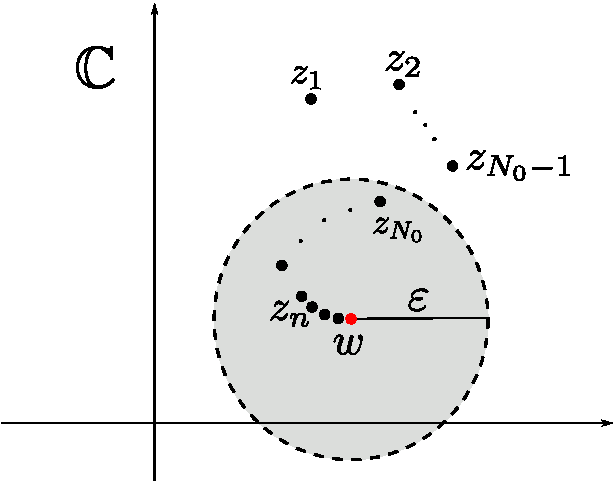
\includegraphics[scale=0.6]{Figuras/fig-sequencia-convergente}
\caption{Definição de limite de uma sequência. Neste figura podemos ver que para $\varepsilon>0$ escolhido, todos os elementos da sequência $(z_n)_{n\in\mathbb{N}}$ cujos índices são maiores ou iguais a um certo $N_0$, são tais que a distância deles à $w$ é menor do que $\varepsilon$.}
\label{fig-sequencia-cauchy1}
\end{figure}


Uma observação importante. 
Já que o objetivo deste texto é ser um texto introdutório à teoria de funções de uma variável complexa, 
vamos evitar ao máximo trabalhar com a definição rigorosa de limite dada acima. Em alguns poucos 
casos, em que isto não for possível, fornecemos figuras ilustrando os argumentos ou conceitos de forma que 
o leitor seja capaz de absolver boa parte das ideias envolvidas.
 
\begin{lema}
\label{lema-conv-parte-real-im-seq}
Seja $(z_n)_{n\in\mathbb{N}}$ é uma
sequência em $\mathbb{C}$. A sequência $z_n\to w$, quando $n\to \infty$, se e somente
se, as sequências de números reais $(\Re(z_n))_{n\in\mathbb{N}}$ e $(\Im(z_n))_{n\in\mathbb{N}}$ convergem, quando $n\to\infty$. Além do mais,
\[
\lim_{n\to\infty} \Re(z_n) = \Re(w)
\qquad \text{e} \qquad 
\lim_{n\to\infty} \Im(z_n) = \Im(w).
\]
\end{lema} 
%\begin{proof}
%A prova deste lema é uma simples aplicação do 
%Lema \ref{lema-re-im-modulo}, da Desigualdade Triangular (Teorema \ref{teo-des-triang})
%e da identidade (I.7) (página \pageref{page:eq-prop-basicas-conjugado}).

%Primeiro assumimos que $z_n\to w$,
%quando $n\to\infty$. 
%Neste caso, temos que 
%\begin{align*}
%\left| 
%\Big(\lim_{n\to\infty}\Re(z_n)\Big) -\Re(w)
%\right|
%&=
%\left| 
%\lim_{n\to\infty}\big(\Re(z_n) -\Re(w)\big)
%\right|
%\\[0.2cm]
%&=
%\lim_{n\to\infty}|\Re(z_n)-\Re(w)|
%\\[0.2cm]
%&=
%\lim_{n\to\infty}|\Re(z_n-w)|
%\\[0.2cm]
%&\leq 
%\lim_{n\to\infty}|z_n-w|
%=
%0,
%\end{align*}
%onde na terceira igualdade usamos que para todo $z,w\in\mathbb{C}$ temos
%$\Re(z)-\Re(w) = \Re(z-w)$. Analogamente provamos a convergência da 
%sequência das partes imaginárias. 

%Reciprocamente, vamos supor que $\Re(z_n)\to a$ e $\Im(z_n)\to b$,
%quando $n\to\infty$. Seja $w=a+ib$. Então para todo $n\in\mathbb{N}$
%temos a seguinte desigualdade 
%\begin{align*}
%|z_n-w|
%&=
%|\Re(z_n)+i\,\Im(z_n) - (a+ib)|
%\\
%&=
%|(\Re(z_n)-a)+i(\Im(z_n)-b)|
%\\
%&\leqslant
%|(\Re(z_n)-a)|+|i(\Im(z_n)-b)|
%\\
%&\leqslant
%|\Re(z_n)-a|+|\Im(z_n)-b|.
%\end{align*} 
%Portanto tomando o limite em ambos os lados verificamos que 
%\[
%\lim_{n\to\infty}|z_n-w|
%\leqslant 
%\lim_{n\to\infty}|\Re(z_n)-a| + 
%\lim_{n\to\infty}|\Im(z_n)-b|
%=0.
%\]

%\end{proof}

Uma grande dificuldade que enfrentamos para trabalhar com o conceito de limite é que, em geral,
não é fácil determinar o ponto para onde nossa sequência converge, mesmo sabendo \textit{a priori} que ela é 
convergente. Por esta razão é conveniente ter em mãos outras condições equivalente para facilitar nossa
tarefa. Uma das mais famosas e utilizadas caracterizações de convergência é a 
de sequências de Cauchy. 

\begin{definicao}\label{def-seq-Cauchy}
\index{Sequência!de Cauchy}
Dizemos que uma sequência $(z_n)_{n\in\mathbb{N}}$ é uma sequência de Cauchy se 
para todo $\varepsilon>0$ dado existe $N_0\in\mathbb{N}$ tal que para todo $m,n\geqslant N_0$
temos 
\[
|z_n-z_m|<\varepsilon.
\]
\end{definicao}
\begin{figure}[h]
\centering
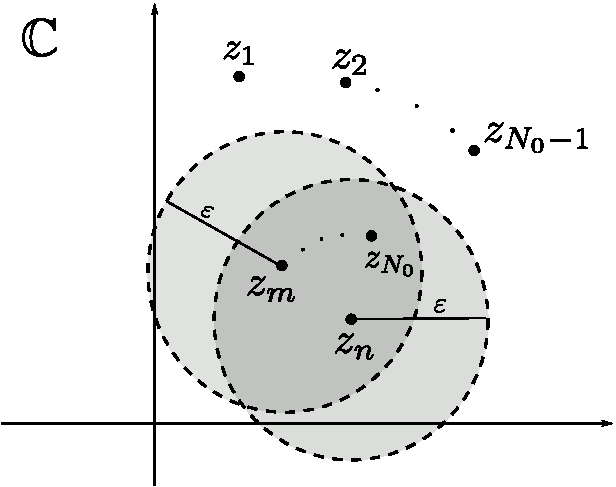
\includegraphics[scale=0.6]{Figuras/fig-sequencia-Cauchy-2}
\caption{Sequência de Cauchy. Segundo a definição para uma sequência ser uma sequência de Cauchy dado $\varepsilon>0$
é possível encontrar um índice $N_0$ tal que se $m$ e $n$ são ambos maiores ou iguais a $N_0$ então 
a distância entre $z_n$ e $z_m$ é no máximo $\varepsilon$. Em outras palavras, para índices suficientemente
grandes os todos os elementos estarão $\varepsilon$-próximos um dos outros.}
\label{fig:fig-sequencia-cauchy}
\end{figure}


Um fato muito importante sobre o conjunto dos números reais é que ele munido de suas operações usuais 
forma um \textit{corpo ordenado} e \textit{completo}.
O adjetivo completo, significa que toda sequência de Cauchy de números reais é convergente
e vice-versa. Como consequência de $\mathbb{R}$ ser completo e das
partes reais e imaginárias serem limitadas por $|z|$, 
segue que $\mathbb{C}$ também é completo. 
De fato, seja $(z_n)_{n\in\mathbb{N}}$ uma sequência de Cauchy em $\mathbb{C}$.  
Nosso primeiro passo é mostrar que a limitação das partes real
e imaginária pode ser usada para mostrar
que as sequências de números reais $(\Re(z_n))_{n\in\mathbb{N}}$ e $(\Im(z_n))_{n\in\mathbb{N}}$
são sequências de Cauchy em $\mathbb{R}$. Já que $(z_n)_{n\in\mathbb{N}}$ uma sequência de Cauchy em $\mathbb{C}$,
sabemos que para qualquer $\varepsilon>0$, existe um $N_0\in\mathbb{N}$ tal que para todo $n,m\geqslant N_0$
temos $|z_n-z_m|<\varepsilon$. Pela limitação das partes real
e imaginária, temos então que 
\begin{align*}
|\Re(z_n)-\Re(z_m)| = |\Re(z_n-z_m)|\leqslant |z_n-z_m|<\varepsilon
\\[0.2cm]
|\Im(z_n)-\Im(z_m)| = |\Im(z_n-z_m)|\leqslant |z_n-z_m|<\varepsilon.
\end{align*}
Mostrando que as partes real e imaginária da sequência $(z_n)_{n\in\mathbb{N}}$ são 
ambas sequências de Cauchy. Como $\mathbb{R}$ é completo então cada uma destas sequências 
é convergente, isto é, existem $x,y\in\mathbb{R}$ tais que 
\[
x=\lim_{n\to\infty} \Re(z_n) \qquad \text{e}\qquad 
y=\lim_{n\to\infty} \Im(z_n).
\]
Ainda resta mostrar que $z_n$ converge para $z=x+iy$, quando $n\to\infty$. 
Mas para basta aplicar o Lema \ref{lema-conv-parte-real-im-seq}.

\subsection{Topologia no Plano Complexo}

Vamos voltar nossa atenção agora para alguns conceitos topológicos que serão necessários
para o desenvolvimento do nosso estudo. A maioria das conceitos deve ser razoavelmente 
familiar para a maioria dos estudantes de cálculo e portanto não serão muito novos e
podem ser visto apenas como os antigos mas apresentados em um novo vocabulário. 


\medskip 

Dado um ponto $z\in\mathbb{C}$ e $r>0$ definimos o {\bf disco aberto} de centro 
$z$ e raio $r$, notação $D(z,r)$,
como sendo o conjunto de todos os números complexos que estão a distância no máximo $r$ de $z$,
isto é, $D(z,r) \equiv \{w\in\mathbb{C}: |z-w|<r \}$.
\index{Disco!aberto}
Definimos o {\bf disco fechado} de centro $z$ e raio $r$, notação $\overline{D}(z,r)$, 
como sendo o conjunto de todos os números complexos que estão a distância menor ou igual a $r$ 
do número complexo $z$, isto é, $\overline{D}(z,r)\equiv \{w\in\mathbb{C}: |w-z|\leqslant r\}$.
\index{Disco!fechado}
A fronteira de ambos $D(z,r)$ e $\overline{D}(z,r)$ é definida como sendo o conjunto 
de todos os pontos do plano complexo que estão a distância exatamente $r$ do ponto $z$,
isto, $\{w\in \mathbb{C}: |w-z|=r\}$. Este conjunto será denotado, em geral, por $\partial D(z,r)$, 
mas caso seja conveniente também podemos denotá-lo por $\partial \overline{D}(z,r)$. 
Como o disco aberto de centro zero e raio um irá desempenhar um papel de destaque neste texto,
vamos reservar uma notação especial para este conjunto. Ao invés de usar a notação $D(0,1)$
vamos nos referir a este disco pela notação $\mathbb{D}$, isto é $\mathbb{D}\equiv \{w\in \mathbb{C}: |w|<1\}$.
O conjunto $\mathbb{D}$ também será chamado as vezes de disco unitário.
\index{Disco!unitário}


\begin{figure}[h]
\centering
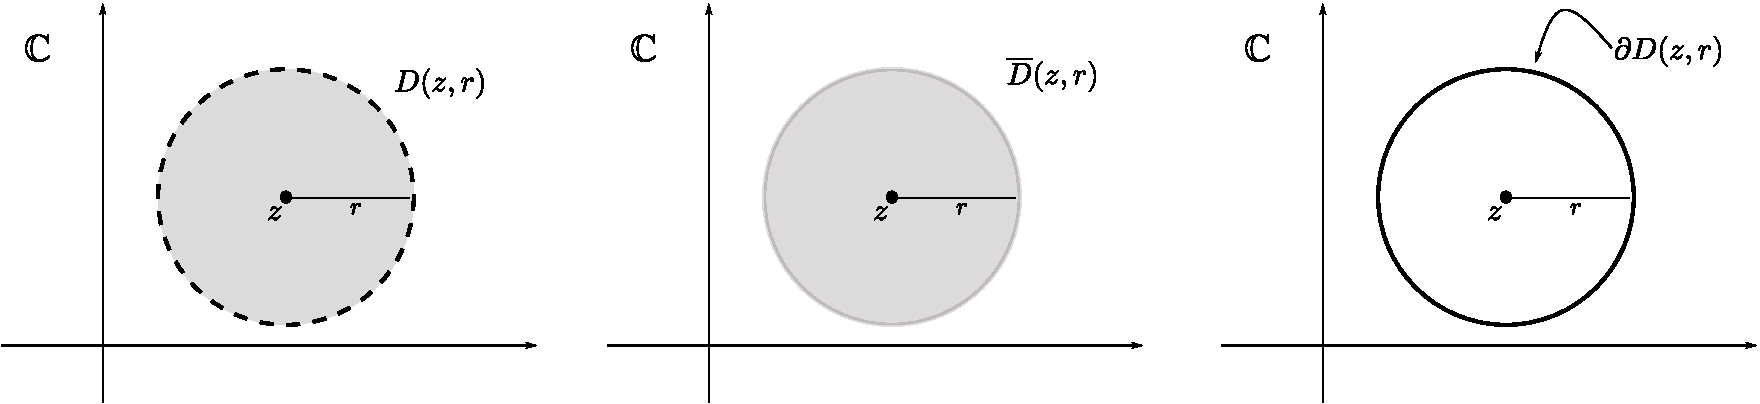
\includegraphics[width=1\linewidth]{Figuras/discos-fronteira}
\caption{Os dicos abertos e fechados de centro $z$ e raio $r>0$ e a fronteira destes discos.}
\label{fig:discos-fronteira}
\end{figure}


\medskip 

Dado um conjunto $U\subset \mathbb{C}$ vamos dizer que $z\in U$ é um {\bf ponto interior} de $U$
\index{Ponto!interior}
se existe algum $r>0$ tal que o disco aberto $D(z,r)$ esteja inteiramente contido em $U$ ou 
em outras palavras $D(z,r)\subset U$. 
O conjunto de todos os pontos interiores de $U$
\index{Interior!de um conjunto}
será denotado por $\mathrm{int}(U)$ e chamado de \textbf{interior de} $U$.
Dizemos que um conjunto $U\subset \mathbb{C}$ é um {\bf conjunto aberto} se todo ponto $z\in U$ é 
\index{Conjunto!aberto}
um ponto interior de $U$. 
Equivalentemente, um subconjunto $U\subset\mathbb{C}$ é aberto se, e somente se, 
$\mathrm{int}(U)=U$.

\begin{figure}[h]
\centering
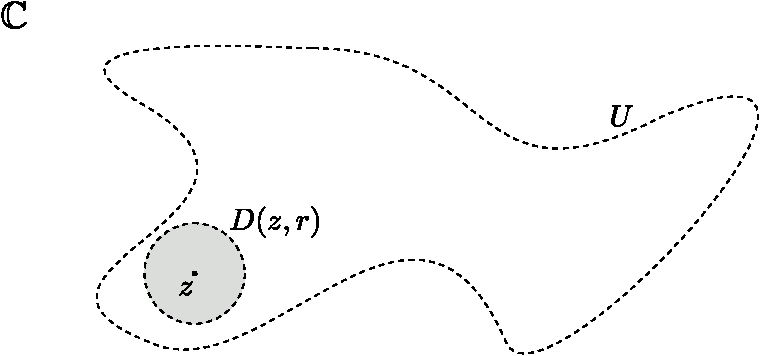
\includegraphics[scale=0.8]{Figuras/ponto-interior}
\caption{Nesta figura $z$ representa um ponto interior de um subconjunto $U\subset \mathbb{C}$.}
\label{fig:ponto-interior}
\end{figure}


Observe que esta definição de conjunto aberto do plano complexo é totalmente semelhante a definição de 
conjunto aberto em $\mathbb{R}^2$. É conveniente usar a convenção que o conjunto vazio é um conjunto aberto.
Observamos que existem diversos subconjuntos $B\subset \mathbb{C}$ com interior vazio, isto é, 
$\mathrm{int}(B)=\empty$. Mesmo assim é sempre verdade que $\mathrm{int}(B)$ é um conjunto
aberto, qualquer que seja $B\subset \mathbb{C}$. 

\medskip 

Um conjunto $F\subset V$ é dito {\bf conjunto fechado} se seu 
complementar $F^c\equiv \mathbb{C}\setminus F \equiv \{z\in \mathbb{C}: z\notin F\}$
\index{Conjunto!fechado}
é um conjunto aberto. 
Já que convencionamos que o conjunto vazio é aberto e já que todo o plano complexo $\mathbb{C}$
também é um conjunto aberto, então o complementar do vazio que é igual a todo plano complexo $\mathbb{C}$ é
um conjunto fechado; bem como o complementar de $\mathbb{C}$ que é igual ao conjunto vazio também é um conjunto
fechado. Podemos mostrar que os únicos subconjuntos de $\mathbb{C}$ que são simultaneamente abertos e fechados
são apenas: $\emptyset$ (conjunto vazio) e $\mathbb{C}$.

Um fato muito importante sobre os conjuntos fechados de $\mathbb{C}$ é que eles 
podem ser completamente caracterizados por sequências. Para isto precisamos de mais uma definição.
Um ponto $z\in\mathbb{C}$ é chamado de {\bf ponto de acumulação}\index{Ponto!de acumulação} de
um subconjunto $B\subset\mathbb{C}$ se existe uma sequência $(z_n)_{n\in\mathbb{N}}$
tal que para todo $n\in\mathbb{N}$ temos: $z_n\in B$ e $z_n\to z$,
quando $n\to\infty$. 


Um ponto $z\in B$ é chamado de {\bf ponto isolado}\index{Ponto!isolado} 
se existe algum $r>0$ de forma que $D(z,r)\cap B = \{z\}$. Ou seja um ponto $z$ de um conjunto $B$
é um ponto isolado se existe um disco de centro em $z$ e raio $r>0$ tal que 
o único ponto de $B$ que está dentro deste disco aberto é o próprio ponto $z$.

\begin{proposicao}\label{prop-caract-fechados-sequencias}
Um subconjunto não-vazio $F\subset\mathbb{C}$ é um conjunto fechado se, e somente se, todo ponto 
de acumulação de $F$ pertence a $F$. 
\end{proposicao}
Já que o complementar de um conjunto fechado é um conjunto aberto segue da proposição 
acima que os conjuntos abertos também podem ser completamente caracterizados 
por sequências.

\medskip 

O {\bf fecho}\index{Fecho} de um subconjunto arbitrário $B\subset \mathbb{C}$ é definido como sendo 
a união de todos os pontos de acumulação do conjunto $B$. O fecho de $B$ é denotado por $\overline{B}$. 
Note que se $B\neq \emptyset$, então $\overline{B}\neq \emptyset$. Além do mais 
qualquer que seja $B\subset\mathbb{C}$ temos sempre $B\subset \overline{B}$.
O leitor é convidado a verificar que o fecho do disco aberto de centro $z$ e raio $r>0$
é exatamente o disco fechado de centro $z$ e raio $r$.

\medskip 

Dado um subconjunto arbitrário $B\subset \mathbb{C}$ definimos a {\bf fronteira}\index{Fronteira} de $B$
como sendo o conjunto $\partial B \equiv \overline{B}\setminus \mathrm{int}(B)$.
Em outras palavras, $\partial B$ é o conjunto formado por todos os pontos do fecho de $B$
que não pertencem ao interior de $B$. 
Convidamos o leitor a pensar em exemplos de subconjuntos de $\mathbb{C}$ 
que possuem fronteira vazia. 
Note que as definições de fronteira de discos (abertos e fechados) dada anteriormente 
coincidem com a noção de fronteira definida neste parágrafo. 


\begin{figure}
\centering
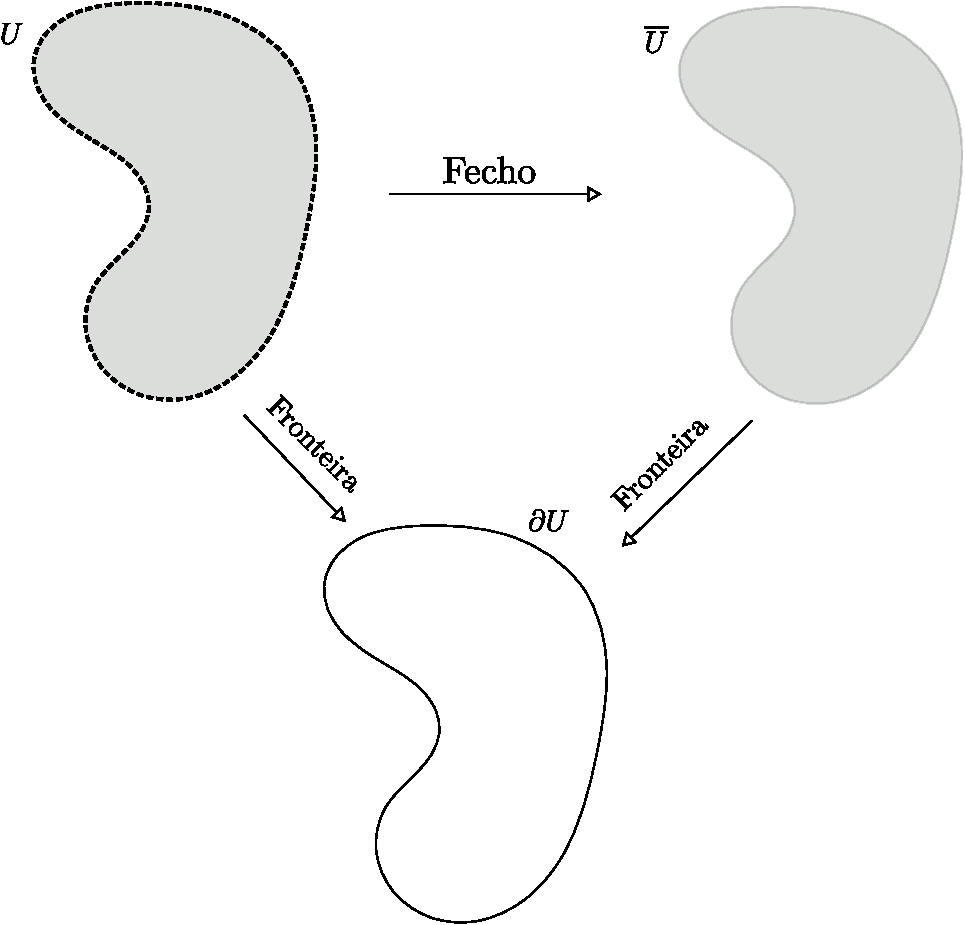
\includegraphics[width=0.7\linewidth]{Figuras/fecho-fronteira}
\caption{A esquerda um subconjunto $U$ do plano complexo. A direita o fecho e em baixo a fronteira de $U$.
Esta figura também destaca que $\partial U = \partial \overline{U}$.}
\label{fig:fecho-fronteira}
\end{figure}


\medskip 
Um subconjunto $B\subset \mathbb{C}$ é chamado de {\bf conjunto limitado}\index{Conjunto!limitado} 
se existe algum número real (finito) $r>0$ tal que 
$B\subset D(0,r)$, isto é, $B$ é limitado se ele está inteiramente contido em um disco de raio
$r>0$. Alternativamente, $B$ é limitado se existe $r>0$ tal que 
para todo $z\in B$ temos que  $|z|<r$. Se $B\subset \mathbb{C}$ é um conjunto limitado,
então definimo o {\bf diâmetro} de $B$ como sendo o número real 
\[
\mathrm{diam}(B) \equiv \sup_{z,w\in B}|z-w|,
\] 
onde ``$\sup$'' denota o supremo do conjunto de todas as distâncias $|z-w|$ com $z$ e $w$
variando por todo conjunto $B$. A única propriedade que vamos precisar nesta seção sobre
supremo é que se $z$ e $w$ são dois pontos arbitrários em $B$ então a seguinte desigualdade é satisfeita
\[
|z-w|\leqslant \mathrm{diam}(B).
\]
%Veja o Apêndice \ref{Apend-sup-inf}, para maiores detalhes
%sobre a definição precisa e propriedades básicas de supremos.


\medskip

Finalmente estamos prontos para apresentar uma das noções mais importantes desta seção
que é a noção de compacidade. Dizemos que um subconjunto $K\subset \mathbb{C}$ é um 
{\bf conjunto compacto}\index{Conjunto!compacto} se $K$ é ao mesmo tempo um conjunto 
fechado e limitado. 

Existe uma caracterização, muito importante, dos compactos de $\mathbb{C}$ 
em termos de sequências. Para enunciarmos este resultado precisamos antes da definição 
do que é uma subsequência.\index{Subsequência}

Uma {\bf subsequência}\index{Subsequência} de uma 
sequência $(z_n)_{n\in\mathbb{N}}\equiv \{z_1,z_2,z_3,\ldots\}$ de números complexo 
é simplesmente uma sequência $(z_{n_k})_{k\in\mathbb{N}}$ construída selecionando-se da sequência original
somente os elementos de índice $1\leqslant n_1<n_2<n_3<\ldots$, onde $(n_k)_{k\in\mathbb{N}}$ pode ser escolhida como 
sendo qualquer sequência infinita estritamente crescente de números naturais.

Por exemplo, $\{z_{4},z_{7},z_{39},z_{100},\ldots\}$ é um exemplo de uma subsequência da 
sequência $\{z_1,z_2,z_3,z_4,\ldots\}$. Neste exemplo $n_1=4, n_2=7, n_3=39, n_4=100$ e assim por diante.
Em geral, qualquer função estritamente crescente $f:\mathbb{N}\to\mathbb{N}$ 
determina uma subsequência e vice-versa. Mais precisamente, dada uma sequência 
$(z_n)_{n\in\mathbb{N}}\equiv\{z_1,z_2,z_3,\ldots\}$ a subsequência determinada por $f$ é 
definida como sendo a sequência $\{z_{f(1)},z_{f(2)},z_{f(3)},\ldots\}$. 
Esta subsequência é denotada por $(z_{f(n)})_{n\in\mathbb{N}}$. Apesar de ser bastante
clara e sugestiva, esta notação é menos usada que a notação anterior $(z_{n_k})_{k\in\mathbb{N}}$.
Mas elas podem ser encaradas do mesmo ponto de vista pensando que $n_k=f(k)$, para todo $k\in\mathbb{N}$,
para alguma função $f:\mathbb{N}\to\mathbb{N}$ estritamente crescente. 
Um fato importante de se observar é que, vista como um conjunto, uma subsequência deve ser sempre 
um subconjunto da sequência original, isto é, $(z_{n_k})_{k\in\mathbb{N}}\equiv \{z_{n_1},z_{n_2},\ldots\}
\subset \{z_1,z_2,\ldots\}\equiv (z_n)_{n\in\mathbb{N}}$. Uma grande vantagem da notação 
$(z_{n_k})_{k\in\mathbb{N}}$ é que 
se quisermos considerar uma subsequência desta subsequência, 
basta modificar a notação acrescentando mais um subíndice ficando, por exemplo, 
com $(z_{n_{k_{p}}})_{p\in\mathbb{N}}$, onde fica subentendido que $k_1<k_2<k_3\ldots$ e  
$\{n_{k_1},n_{k_2},\ldots\}\subset \{n_1,n_2,\ldots\}$.


\begin{teorema}
Um conjunto $K\subset \mathbb{C}$ é compacto se, e somente se, toda sequência $(z_n)_{n\in\mathbb{N}}$
contida em $K$, possui alguma subsequência que converge para algum ponto pertencente a $K$.
\end{teorema}

% \begin{proof}
% Vamos mostrar primeiro que se $K$ é compacto então qualquer sequência $(z_n)_{n\in\mathbb{N}}$
% contida em $K$, possui alguma subsequência convergente.
% Para isto vamos considerar as seguintes duas sequências de números reais associadas à $(z_n)_{n\in\mathbb{R}}$ dadas por
% \begin{align*}
% x_n \equiv \Re(z_n) \qquad\text{e}\qquad y_n\equiv \Im(z_n).
% \end{align*}
% Já que estamos assumindo que $K$ é compacto e $(z_n)_{n\in\mathbb{N}}$
% está contida em $K$, então $K$ é limitado. Assim existe 
% $r>0$ tal que $|z_n|<r$. Aplicando o Lema \ref{lema-re-im-modulo} 
% concluímos que $|x_n|< r$ e $|y_n|< r$, para todo $n\in\mathbb{N}$. 
% Agora usamos o fato que toda sequência de números reais limitada, possui
% uma subsequência convergente. Logo existe uma subsequência $(x_{n_k})_{k\in\mathbb{N}}$ 
% tal que $x_{n_k}\to x$ quando $k\to\infty$. Agora olhamos para a 
% subsequência $(y_{n_k})_{k\in\mathbb{N}}$. Já que ela é uma subsequência de $(y_n)_{n\in\mathbb{N}}$ então 
% ela é limita. Portanto podemos garantir que ela possui 
% uma subsequência $(y_{n_{k_p}})_{p\in\mathbb{N}}$ tal que $y_{n_{k_p}}\to y$, quando $p\to\infty$.  
% Note que $x_{n_{k_p}}\to x$, quando $p\to\infty$ uma vez que qualquer subsequência de uma sequência 
% convergente também é convergente e o limite é o mesmo. 
% Para finalizar esta parte da prova vamos mostrar que $(z_{n_{k_p}})_{p\in\mathbb{N}}$ converge
% para $z=x+iy$, quando $p\to\infty$. De fato, pela desigualdade triangular temos que 
% \begin{align*}
% \lim_{k\to\infty} |z_{n_{k_p}} -z |
% &=
% \lim_{k\to\infty} |\Re(z_{n_{k_p}})+i\Im(z_{n_{k_p}}) - (x+iy)|
% \\
% &=
% \lim_{k\to\infty} |x_{n_{k_p}}+iy_{n_{k_p}} - (x+iy)|
% \\
% &=
% \lim_{k\to\infty} |x_{n_{k_p}}+iy_{n_{k_p}} - (x+iy)|
% \\
% &=
% \lim_{k\to\infty} |(x_{n_{k_p}}-x)+i (y_{n_{k_p}}-y)|
% \\
% &\leqslant 
% \lim_{k\to\infty} |(x_{n_{k_p}}-x)|
% +
% \lim_{k\to\infty} |(y_{n_{k_p}}-y)|=0.
% \end{align*}

% Vamos mostrar agora que se $K$ tem a propriedade de que qualquer sequência em $K$ possui 
% subsequência que converge para um ponto em $K$, então $K$ é limitado e fechado. 


% Suponha por absurdo que $K$ não é limitado.
% Então para cada $n\in\mathbb{N}$ existe $z_n\in K$ tal que $n<|z_n|$. Logo qualquer subsequência
% $(z_{n_k})_{k\in\mathbb{N}}$ satisfaz $n_k<|z_{n_k}|$ e portanto não converge o que é um absurdo.


% Resta mostrar que $K$ é fechado. Pela Proposição \ref{prop-caract-fechados-sequencias} 
% sabemos que isto é equivalente a mostrar que $K$ possui todos seus pontos de acumulação,
% isto é, $K=\overline{K}$. 
% Seja $z\in \overline{K}$. Então pela definição do fecho de $K$, podemos afirmar que 
% existe uma sequência $(z_n)_{n\in\mathbb{N}}$ tal que $z_n\in K$ para todo $n\in\mathbb{N}$ 
% e além do mais $z_n\to z$. Já que a sequência $(z_n)_{n\in\mathbb{N}}$ é convergente, qualquer
% de suas subsequências também convergem e para o mesmo limite, que no caso é $z$.
% Da propriedade do nosso conjunto $K$ existe pelo menos uma subsequência 
% $(z_{n_{k}})_{k\in\mathbb{N}}$
% que converge para um ponto de $K$, mas como acabamos de mencionar o limite desta subsequência é 
% exatamente $z$ e portanto pela nossa hipótese, este deve ser um ponto de $K$. O que mostra que 
% todo ponto de $\overline{K}$ é também um ponto de $K$, isto é, $\overline{K}\subset K$.
% Mas por outro lado, sabemos que a inclusão reversa $K\subset \overline{K}$ é sempre válida para qualquer 
% conjunto. Logo $K=\overline{K}$ e portanto $K$ é fechado e isto encerra a prova do teorema.
% \end{proof}



Outra propriedade importante sobre conjuntos compactos, que é usada na prova do importante
Teorema de Cauchy-Goursat, é enunciada no teorema abaixo. 

\begin{teorema}[Teorema de Cantor]
Para cada $n\in\mathbb{N}$ seja $K_n\subset \mathbb{C}$ um conjunto compacto não-vazio. Suponha que $K_{n}\supset K_{n+1}$ e $\mathrm{diam}(K_n)\to 0$, quando $n\to\infty$. Então existe um único ponto $z\in\mathbb{C}$ tal que $z\in K_n$ para todo $n\in\mathbb{N}$, ou seja, 
\[
z\in \bigcap_{n=1}^{\infty} K_n.
\]


\end{teorema}

\begin{proof}
Já que para cada $n\in\mathbb{N}$ estamos assumindo que $K_n$ é não-vazio, então existe algum
$z_n\in K_n$. Como $\mathrm{diam}(K_n)\to 0$ temos que a sequência $(z_n)_{n\in\mathbb{N}}$
é uma sequência de Cauchy. 

\begin{figure}[h]
\centering
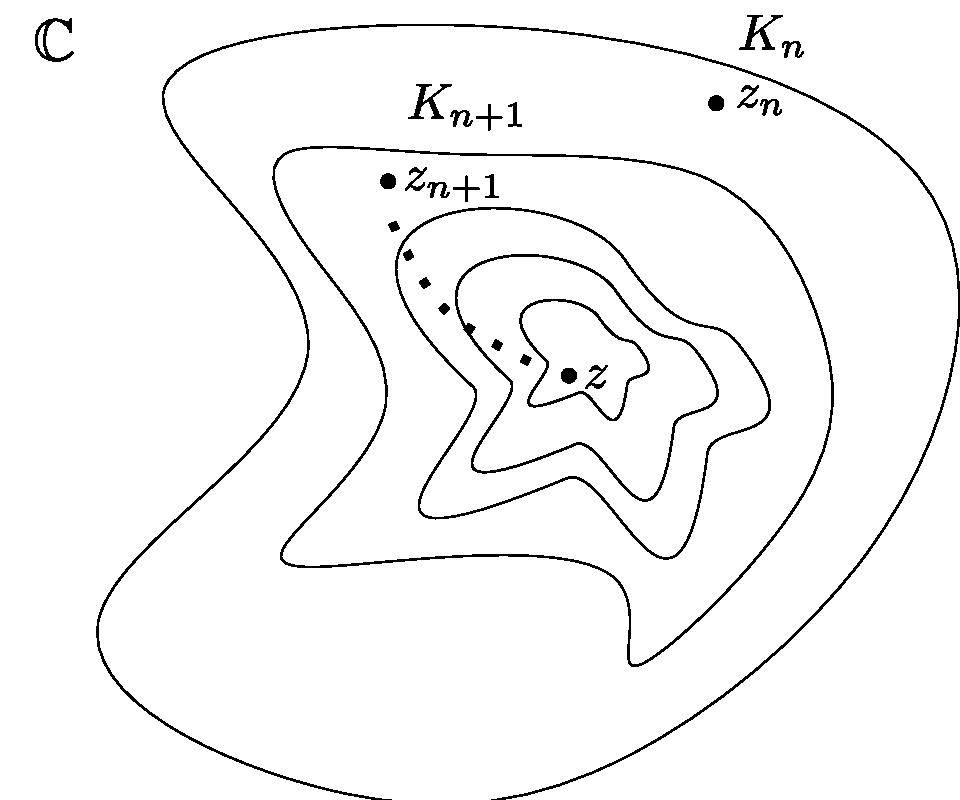
\includegraphics[scale=0.6]{Figuras/teorema-cantor}
\caption{A construção da sequência $(z_n)_{n\in\mathbb{N}}$.}
\label{fig:teorema-cantor}
\end{figure}


De fato, já que $\mathrm{diam}(K_n)\to 0$ sabemos que para qualquer $\varepsilon>0$ vai existir existe $N_0\in\mathbb{N}$ tal que se $n\geqslant N_0$ então 
$\mathrm{diam}(K_n)<\varepsilon$. Por hipótese, 
para qualquer $j\geqslant N_{0}$ temos $K_{N_0}\supset K_{j}$
e portanto os pontos $z_n$ e $z_{m}$ pertencem a $K_{N_0}$. 
Desta observação e da definição de supremo segue
que $|z_n-z_m|\leq \mathrm{diam}(K_n)<\varepsilon$
para todo $m,n\geqslant N_0$ mostrando assim que $(z_n)_{n\in\mathbb{N}}$
é uma sequência de Cauchy. Como $\mathbb{C}$ é completo. Sabemos que existe $z\in\mathbb{C}$
tal que $z_n\to z$, quando $n\to\infty$. Como para cada $n\in\mathbb{N}$ temos que $K_n$ é compacto e $\{z_n,z_{n+1},\ldots\}$
é uma sequência em $K_n$. Então $z=\lim_{n\to\infty} z_n$ também pertence a $K_n$.
Portanto $\cap_{n=1}^{\infty}K_n$ é não-vazio. Para mostrar que $z$ é o único ponto 
que pertence a esta interseção infinita argumentamos por absurdo. Suponha que exista $z'\in \cap_{n=1}^{\infty}K_n$ com $z'\neq z$. Então $|z'-z|>0$. Por outro lado, como $z,z'\in K_n$ 
para todo $n\in\mathbb{N}$ logo
\[
0<|z-z'|\leqslant \mathrm{diam}(K_n), \qquad \forall n\in\mathbb{N}
\]
o que é um absurdo já que $\lim_{n\to\infty}\mathrm{diam}(K_n)=0$.
\end{proof}

\subsection{Conjuntos Conexos e Domínios}
\label{subsec-coonj-conexos-dominios}

A última noção de topologia que vamos precisar é a de conexidade. 
Um conjunto $B\subset \mathbb{C}$ é dito {\bf conexo}\index{Conjunto!conexo} 
se não é possível encontrar dois subconjuntos do plano complexo $U$ e $V$ abertos, 
disjuntos ($U\cap V = \emptyset)$, não-vazios e tais que: 
\begin{itemize}
	\item $B\cap U\neq \emptyset$;  
	\item $B\cap V\neq \emptyset$; e
	\item $B\subset V\cup U$.
\end{itemize}

\begin{figure}[h]
\centering
\includegraphics[width=0.9\linewidth]{"Figuras/fig-conjuntos-conexos"}
\caption[Conjunto Conexo]{Exemplo de um conjunto $B$ conexo. No lado esquerdo da figura temos um exemplo de um conjunto conexo $B$. 
No lado direito, podemos ver que o $B$ não pode ser separado 
por abertos $U$ e $V$ não-vazios, disjuntos, ambos interceptando $B$, e que cobrem $B$ ($B\subset U\cup V$).
Informalmente, vemos que $B$ não pode ser separado em dois pedaços (em que cada pedaço é um 
conjunto aberto). }
\label{fig:conjuntos-conexos}
\end{figure}


Esta definição de conexidade, formaliza, em um grande número de casos, a ideia do que seria 
um subconjunto do plano complexo formado por apenas um ``pedaço''. 
Excetuando alguns casos patológicos como, por exemplo, 
o do conjunto mostrado na Figura \ref{fig-pente}, podemos pensar em um 
conjunto conexo como sendo realmente um conjunto formado por um único ``pedaço''. 
Este é o caso quando o conjunto em questão é um \textit{domínio}.  


Na figura abaixo temos um exemplo simples de um conjunto $B$ que não é conexo.
Às vezes, nos referimos a tais conjuntos como desconexos. 


\begin{figure}[h]
\centering
\includegraphics[width=0.9\linewidth]{"Figuras/fig-conjunto-desconexo"}
\caption[Conjunto Conexo]{Exemplo de um conjunto $B$ que é desconexo. 
O conjunto $B$, formado pela união dos pontos pertencentes às duas regiões pintadas na
cor cinza escuro, no lado esquerdo da figura acima, é um exemplo de um conjunto que não é conexo. 
A direita mostramos como é possível separar $B$ 
por abertos $U$ e $V$ disjuntos não-vazios que: ambos interceptam $B$; e o cobrem.}
\label{fig:conjunto-desconexo}
\end{figure}


Um subconjunto $U\subset\mathbb{C}$ que é ao mesmo tempo aberto e conexo, 
será chamado de 
{\bf domínio}\index{Domínio}. Na próxima seção vamos mostrar que 
um domínio $U\subset \mathbb{C}$ por ser caracterizado pelos
caminhos existente nele. 



\section{Caminhos no Plano Complexo}

\begin{definicao}[Caminho Suave]\label{def-caminho-em-C}
Seja $I=[a,b]\subset\mathbb{R}$ um intervalo não degenerado, isto é, $a<b$. 
Um caminho suave\index{Caminho!suave} 
em $\mathbb{C}$ é uma aplicação $\gamma:I\to \mathbb{C}$
possuindo derivada contínua em todos os pontos de $I$.
\end{definicao}

Antes de prosseguir devemos fazer algumas observações sobre a definição acima.
Primeira observação é que a condição de diferenciabilidade imposta nesta definição, 
deve ser entendida da seguinte forma.
Para cada $t\in I$ lembre-se que podemos escrever $\gamma(t) = \Re(\gamma(t))+i\Im(\gamma(t))$.
As funções $t\longmapsto \Re(\gamma(t))$ e $t\longmapsto \Im(\gamma(t))$ definem
duas funções reais chamadas de coordenadas do caminho $\gamma$.
Por simplicidade, vamos denotá-las por $x(t)\equiv\Re(\gamma(t))$ e 
$y(t)\equiv\Im(\gamma(t))$. 
Finalmente, a condição de suavidade
é que as funções coordenadas sejam deriváveis e que suas derivadas 
$t\longmapsto x'(t)$ e $t\longmapsto y'(t)$ sejam funções contínuas para todo $a<t<b$ e 
nos pontos $t=a$ e $t=b$ exigimos que os seguintes limites laterais existam e satisfaçam as seguintes
igualdades:
\[
\lim_{t\to a^{+}}x'(t) = x'(a)\equiv\lim_{h\to 0^{+}}\frac{x(a+h)-x(a)}{h}  
\]
e
\[
\lim_{t\to a^{+}}y'(t) = x'(b)\equiv \lim_{h\to 0^{-}}\frac{x(b+h)-x(b)}{h}  
\]

É claro que poderíamos também enunciar a condição de suavidade diretamente para $\gamma$
sem ter que apelar para suas funções coordenadas. Para isto tomaríamos, para cada $t$ no intervalo aberto $(a,b)$
\[
\gamma'(t) = \lim_{h\to 0} \frac{\gamma(t+h)-\gamma(t)}{h}
\]
e similarmente, 
\[
\gamma'(a) = \lim_{h\to 0^{+}} \frac{\gamma(a+h)-\gamma(a)}{h}
\qquad \text{e}\qquad 
\gamma'(b) = \lim_{h\to 0^{-}} \frac{\gamma(b+h)-\gamma(b)}{h}.
\]
Em seguida, exigiríamos que $\gamma'(t)$ variasse continuamente em $[a,b]$.
Esta definição seria mais elegante, mas para torná-la completamente precisa seria necessário antes
atentarmos para um detalhe, ainda não falamos o que é continuidade de funções 
a valores em $\mathbb{C}$. Muito provavelmente 
o leitor já deva estar imaginando que isto será feito com a base na definição de continuidade
de funções tomando valores em $\mathbb{R}^2$, já que na seção passada todos os conceitos topológicos
em $\mathbb{C}$ foram construídos em analogia aos de $\mathbb{R}^2$. 

Considerando então o caminho $\gamma$, como uma função tomando valores em $\mathbb{R}^2$
temos para cada $a<t<b$ a seguinte igualdade 
\begin{align*}
\gamma'(t) 
&= 
\lim_{h\to 0} \frac{\gamma(t+h)-\gamma(t)}{h}
=
\lim_{h\to 0} \frac{1}{h}\big(x(t+h),y(t+h)\big) - \big(x(t),y(t)\big)
\\[0.3cm]
&=
\lim_{h\to 0} \left( \frac{x(t+h)-x(t)}{h},\frac{y(t+h)-y(t)}{h} \right)
\\[0.3cm]
&=
(x'(t),y'(t)).
\end{align*}
Voltando para o plano complexo temos
\[
\gamma'(t) = x'(t)+iy'(t).
\]
De maneira análoga, estendemos a igualdade para os pontos $t=a$ e $t=b$.


\bigskip 

Se $\gamma:I\to\mathbb{C}$ é um caminho suave em $\mathbb{C}$ o ponto
$\gamma(a)$ é chamado de {\bf ponto inicial}\index{Ponto!inicial} 
e $\gamma(b)$ {\bf ponto terminal}\index{Ponto!terminal} do 
caminho $\gamma$. O conjunto imagem do caminho $\gamma$, isto é, 
o conjunto $\gamma(I)\subset\mathbb{C}$ é chamado de {\bf curva} no plano complexo
determinada por $\gamma$.
Em muitas situações abusamos da notação e chamamos a curva determinada por $\gamma$
de caminho $\gamma$. 
Quando $\gamma(a)=\gamma(b)$ dizemos que $\gamma$ é um 
{\bf caminho fechado}\index{Caminho!fechado} ou alternativamente que $\gamma$ é
um curva fechada.

\begin{exemplo}\label{exemplo-param-segreta}
O segmento de reta em $\mathbb{C}$ unindo os pontos quaisquer fixados 
$z_1=x_1+iy_1$ e $z_2=x_2+iy_2$
pode ser visto como um caminho suave representado pela função $\gamma:[0,1]\to\mathbb{C}$
dada por 
\[
\gamma(t) = z_1+t(z_2-z_1) = \big((1-t)x_1+tx_2\big)+i\big((1-t)y_1+ty_2\big).
\] 
\end{exemplo}

\begin{exemplo}\label{exemplo-param-circ}
A fronteira de um disco de centro $z=x+iy$ e raio $r>0$, isto é, $\partial D(z,r)$ 
pode ser vista como a imagem do caminho $\gamma:[0,2\pi]\to\mathbb{C}$ dado por
\[
\gamma(\theta) = z+r(\cos\theta+i\sen\theta) = (x+r\cos\theta)+i(y+r\sen\theta).
\]
\end{exemplo}

Da maneira como introduzimos o conceito de um caminho $\gamma:[a,b]\to\mathbb{C}$, 
temos automaticamente uma maneira de definir sua orientação. 
Intuitivamente, a orientação é dada pelo percurso 
do caminho a medida que o parâmetro $t$ cresce de $a$ para $b$. 
Assim dizemos que o caminho $\gamma$ está orientado do ponto 
inicial $\gamma(a)$ para o ponto terminal $\gamma(b)$. 

Definimos também o caminho reverso\index{Caminho!reverso} do $\gamma:[a,b]\to\mathbb{C}$
pela aplicação $\gamma^{-}:[a,b]\to\mathbb{C}$ dada por 
\begin{align}\label{formula-caminho-reverso}
\gamma^{-}(t) \equiv \gamma(a+b-t), \quad \text{para todo}\ t\in[a,b].
\end{align}
Note que as curvas $\gamma([a,b])$ e $\gamma^{-}([a,b])$ associadas à ambos $\gamma$ e seu reverso, 
são exatamente as mesmas, mas do ponto de vista de caminhos temos que o ponto inicial de um é o ponto 
terminal do outro e vice-versa. 


\begin{figure}[h]
\centering
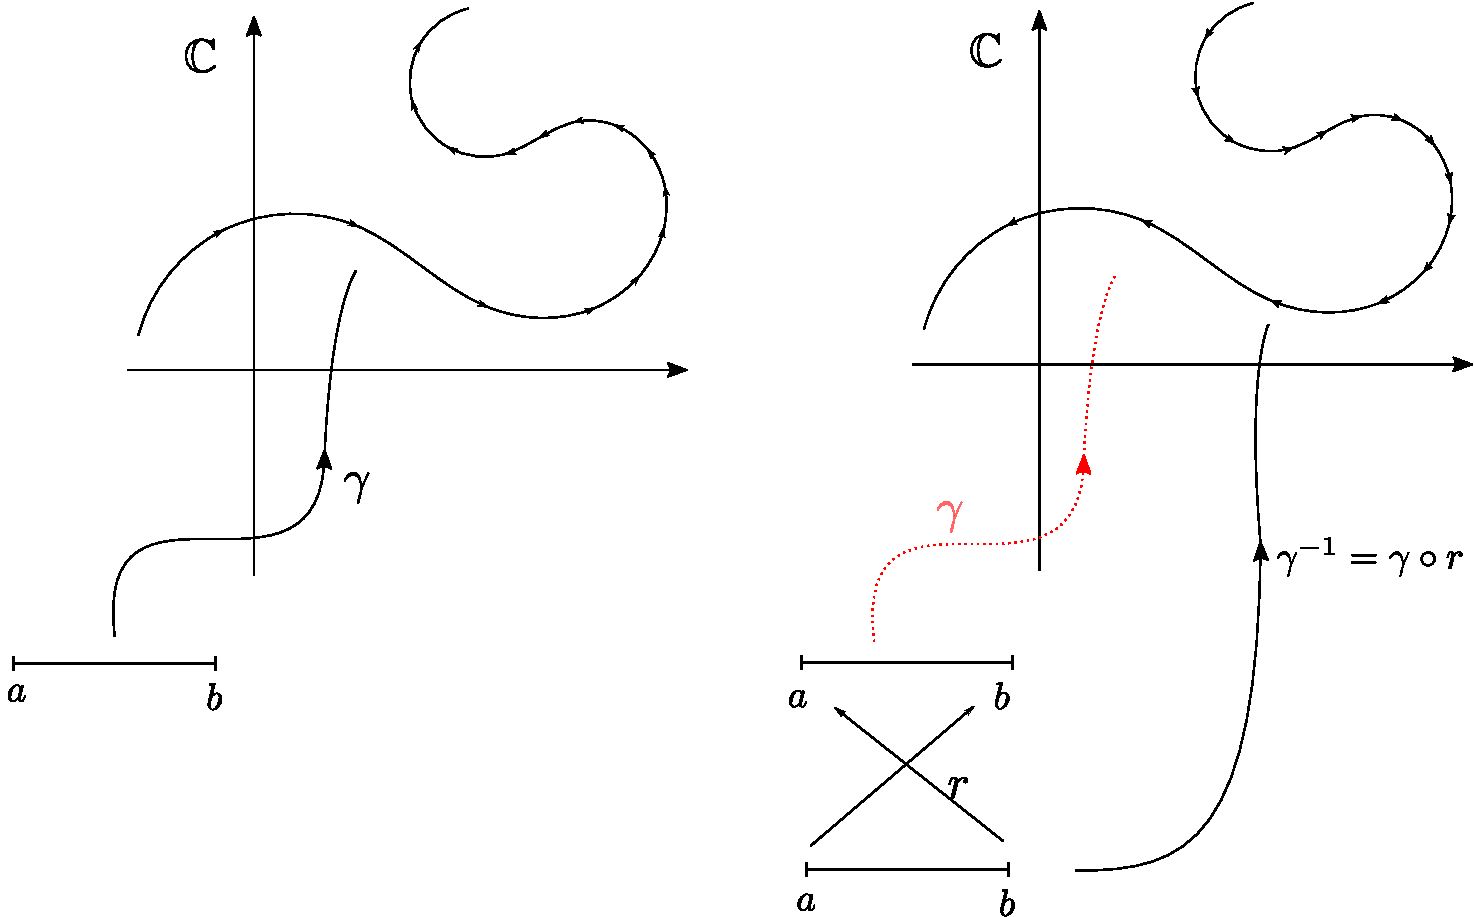
\includegraphics[width=0.9\linewidth]{Figuras/fig-gamma-gamma-reverso}
\caption{Um caminho suave $\gamma:[a,b]\to\mathbb{C}$ e seu reverso $\gamma^{-1}= \gamma\circ r$, onde $r(t)=a+b-t$.
Note que $r$ envia $a$ em $b$ e vice-versa, revertendo assim a orientação do intervalo $[a,b]$ e 
consequentemente o caminho $\gamma$.}
\label{fig-gamma-gamma-reverso}
\end{figure}



Exemplificamos agora como obter os caminhos reversos dos caminhos definidos no exemplos dados
acima.
No Exemplo \ref{exemplo-param-segreta} temos $\gamma(t) = z_1+t(z_2-z_1),\ t\in[0,1]$. Para obter a
expressão de $\gamma^{-1}$ basta aplicar a fórmula \eqref{formula-caminho-reverso} com $a=0$ e $b=1$
obtendo assim $\gamma^{-1}(t) = z_1+(1-t)(z_2-z_1)$. 
No caso do caminho do Exemplo \ref{exemplo-param-circ} temos 
$\gamma(\theta) = z+r(\cos\theta+i\sen\theta),\ t\in[0,2\pi]$. Agora aplicamos a fórmula 
\eqref{formula-caminho-reverso} com $a=0$ e $b=2\pi$ obtendo portanto 
$\gamma^{-1}(\theta) = z+r(\cos(2\pi-\theta)+i\sen(2\pi-\theta)),\ t\in[0,2\pi]$.

\begin{definicao}[Caminho suave por partes]
\label{def-caminho-suave-partes}
\index{Caminho!suave por partes}
Um caminho suave por partes em $\mathbb{C}$ é uma coleção finita de caminhos suaves
$\gamma_{1}:[a_1,b_1]\to\mathbb{C}$, $\gamma_{2}:[a_2,b_2]\to\mathbb{C}$, \ldots, 
$\gamma_{n}:[a_n,b_n]\to\mathbb{C}$, satisfazendo para cada $1\leqslant i\leqslant n-1$
as seguintes relações $\gamma_{i}(b_i)=\gamma_{i+1}(a_{i+1})$.
\end{definicao}


Será conveniente usar a notação $\gamma_1*\gamma_2*\ldots*\gamma_n$ para denotar um caminho suave
por partes $\gamma$ como na definição acima. Analogamente, tal caminho suave por partes é dito
fechado se $\gamma_1(a_1)=\gamma_{n}(b_n)$. Como no caso de caminhos suaves, 
o ponto $\gamma_1(a_1)$ é chamado de ponto inicial e o ponto 
$\gamma_n(b_n)$ é chamado de ponto terminal. 


Por exemplo, podemos ver um polígono de 6 lados cujos vértices são os 
pontos $z_1,z_2,\ldots, z_6\in\mathbb{C}$ mostrados na Figura \ref{fig-polig-6-lados}
como um caminho $\gamma = \gamma_1*\gamma_2*\ldots*\gamma_6$.

\begin{figure}[h]
\centering
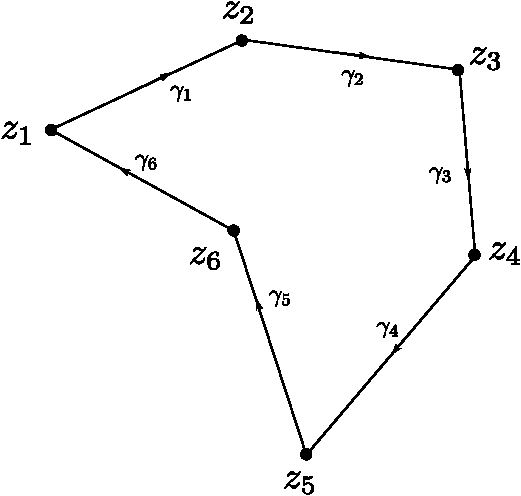
\includegraphics[scale=0.6]{Figuras/fig-polig-6-lados}
\caption{O polígono determinado pelo caminho suave por partes $\gamma= \gamma_1*\ldots*\gamma_6$}
\label{fig-polig-6-lados}
\end{figure}


onde para cada $1\leqslant i\leqslant 6$ temos 
\begin{align*}
\gamma_1(t) = z_1+t(z_2-z_1), \quad t\in [0,1];\\
\gamma_2(t) = z_2+t(z_3-z_2), \quad t\in [0,1];\\
\vdots\qquad \qquad\qquad \qquad \\
\gamma_6(t) = z_6+t(z_1-z_6), \quad t\in[0,1].
\end{align*}

\bigskip 





Em muitas situações é mais conveniente ter os caminhos $\gamma_i$'s de 
$\gamma=\gamma_1*\gamma_2*\ldots*\gamma_n$
parametrizados de forma que seus domínios sejam intervalos ``consecutivos'', isto é, seus pontos
de bordo satisfazem 
\[
a_1<b_1=a_2<b_2=a_3<\ldots<b_{n-1}=a_{n}<b_n.
\]
Mais conveniente ainda é poder trabalhar com caminhos cujos intervalos de definição 
formem uma coleção consecutiva de $n$ subintervalos do intervalo $[0,1]$. 

Dado um caminho suave por partes $\gamma= \gamma_1*\gamma_2*\ldots*\gamma_n$
podemos associar a ele um novo caminho suave por partes 
que será chamado de {\bf normalizado}\index{Caminho!normalizado}.
Para fazer isto, primeiro dividimos o intervalo $[0,1]$ em $n$ subintervalos de
mesmo comprimento
\[
\left[0,\frac{1}{n} \right],
\left[\frac{1}{n},\frac{2}{n} \right],
\ldots
\left[\frac{n-1}{n},1 \right].
\]
Em seguida, para cada $1\leqslant j\leqslant n$, vamos definir uma aplicação bijetiva (afim) 
$r_{j}:[j-1/n,j/n]\to [a_j,b_j]$ que mapeia o subintervalo $[j-1/n,j/n]$ no intervalo $[a_j,b_j]$. 
Esta bijeção é dada por 
\[
r_j(t) = n(b_j-a_j)t-j(b_j-a_j)+b_j, \quad t\in\left[\frac{j-1}{n},\frac{j}{n}\right].
\]
Estas aplicações $r_j$'s são muitas vezes chamadas de re-parametrizações. 
Agora consideramos os caminhos $\gamma_{j}\circ r_j$ com $1\leqslant j\leqslant n$.
Então é fácil ver que $\gamma_{j}\circ r_j$ é um caminho suave em $\mathbb{C}$ e além do 
mais o ponto final de $\gamma_{j-1}\circ r_{j-1}$ coincide com o ponto inicial de 
$\gamma_{j}\circ r_j$. Desta maneira o caminho $\gamma$ pode ser visto como definido 
no intervalo $[0,1]$. 

Dizemos que um caminho suave por partes (normalizado como acima) 
é {\bf simples}\index{Caminho!simples}, se aplicação $\gamma:[0,1]\to\mathbb{C}$ que o define
é injetiva, exceto possivelmente pelos pontos $t=0$ e $t=1$. Mais precisamente, $\gamma(s)\neq \gamma(t)$
para $0\leqslant s<t<1$ e é permitido $\gamma(0)=\gamma(1)$. 
Do ponto de vista geométrico, um caminho simples representa uma curva no plano sem 
auto-interseção, exceto possivelmente pelos pontos inicial e terminal. 


Já temos todos terreno preparado para introduzir uma classe de curvas 
que serão de enorme importância no estudo de integração no plano 
complexo. 

\begin{definicao}
[Curva de Jordan]
\label{def-curva-jordan}
\index{Curva!de Jordan}
Uma curva de Jordan suave por partes é a imagem de um caminho suave por partes, fechado e simples. 
\end{definicao}


\begin{figure}[h]
\centering
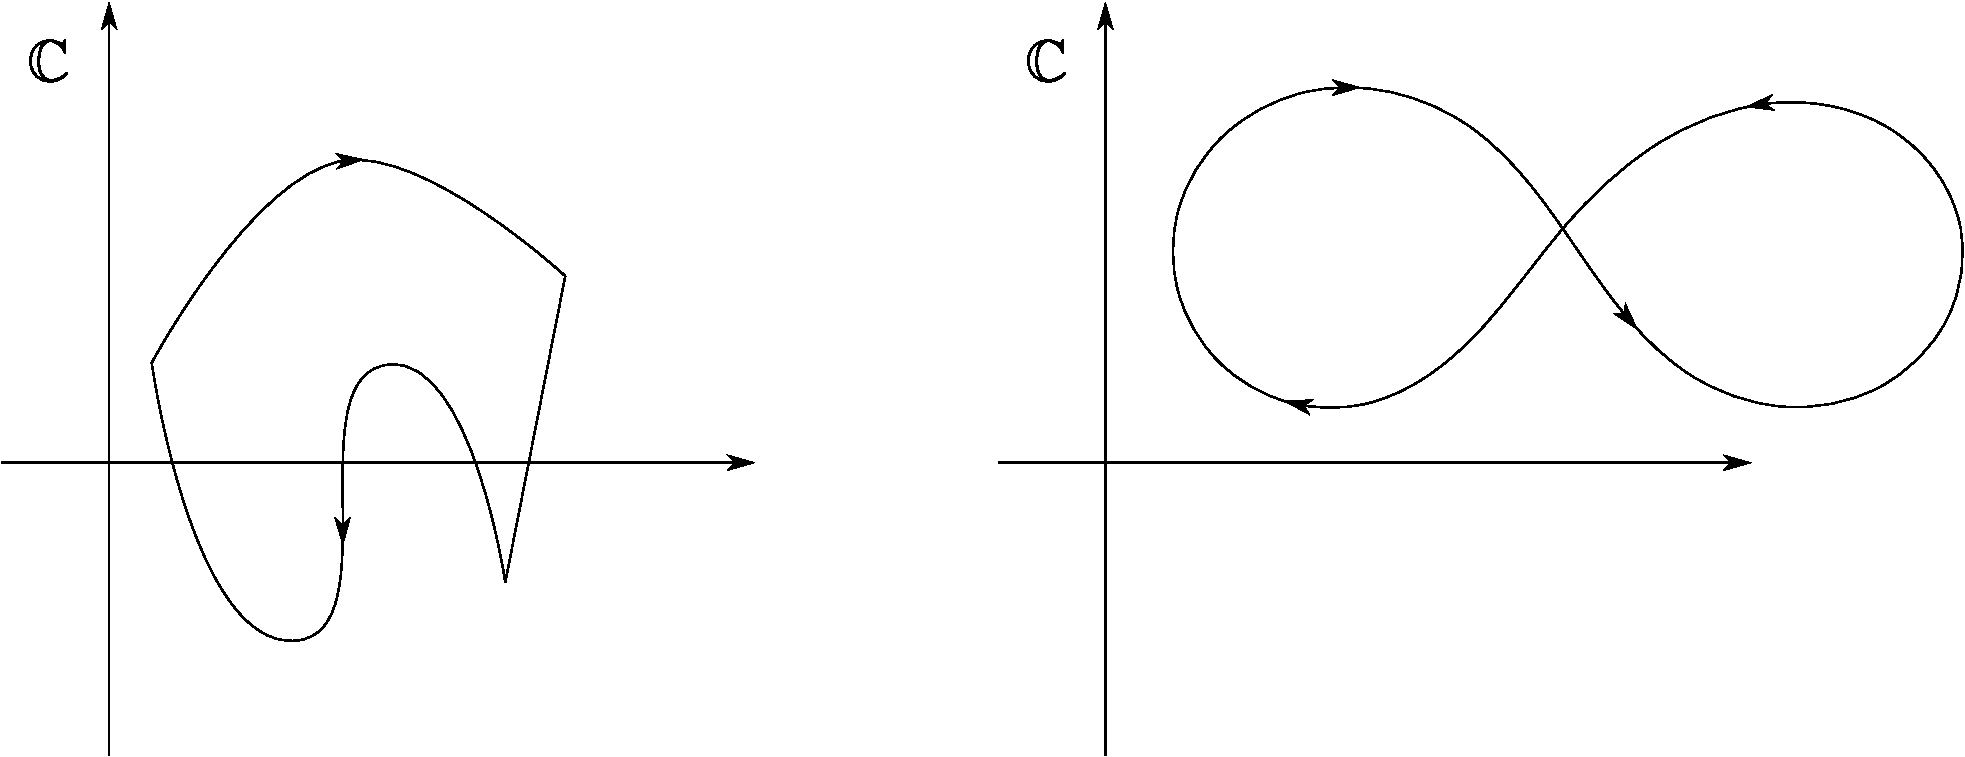
\includegraphics[scale=0.4]{Figuras/fig-curvas-fechadas}
\caption{Caminhos fechados suaves por partes. O caminho da esquerda está associado a uma curva de Jordan. A curva a direita não é uma curva de Jordan pois ela possui um ponto de auto-interseção.}
\label{fig-curvas-fechadas}
\end{figure}



Um dos resultados mais importantes sobre curvas de Jordan é um teorema devido a Jordan.
Ele afirma que uma curva de Jordan suave por partes $\gamma$ divide o plano $\mathbb{R}^2$
em exatamente dois abertos disjuntos, um deles limitado e o outro ilimitado, sendo 
$\gamma$ a fronteira comum entre estes dois abertos. Esse resultado, embora de fácil 
intuição é de demostração bastante elaborada. Atualmente existem vários textos que provam
este teorema. O leitor interessado pode encontrar uma prova deste teorema um pouco 
mais moderna e bem detalhada no Apêndice B da referência \cite{MR1976398}.


\begin{definicao}
\label{def-comp-caminho}
\index{Comprimento!de um caminho}
O comprimento de um caminho suave $\gamma:[a,b]\to\mathbb{C}$ é definido como sendo o número real
\[
\ell(\gamma)\equiv 
\int_{a}^{b} |\gamma'(t)|\, dt.
\]
Se $\gamma$ é um caminho suave por partes da forma $\gamma=\gamma_1*\gamma_2*\ldots*\gamma_n$
então definimos o comprimento de $\gamma$ como sendo $\ell(\gamma)\equiv \ell(\gamma_1)+\ldots+\ell(\gamma_n)$.
\end{definicao}


\begin{exemplo}
Se $\gamma:[0,2\pi]\to\mathbb{C}$ é o caminho dado por $\gamma(\theta)=z+r(\cos\theta+i\sen\theta)$,
com $0\leqslant \theta\leqslant 2\pi$ temos que 
\[
\gamma'(\theta) = \frac{d}{d\theta}[z+r(\cos\theta+i\sen\theta)]=r(-\sen\theta+i\cos\theta).
\]
Portanto $|\gamma'(\theta)|=r$ e assim 
\[
\ell(\gamma) 
= 
\int_{0}^{2\pi} |\gamma'(\theta)|\, d\theta 
= 
r\int_{0}^{2\pi}\, d\theta 
=
2\pi r.
\]
\end{exemplo}

Pensando em um caminho $\gamma:[a,b]\to\mathbb{C}$ como uma função descrevendo a posição de uma partícula
no instante $t$ o número $\ell(\gamma)$ pode ser interpretado como a distância total percorrida pela 
partícula durante o intervalo de tempo $[a,b]$. Portanto se ela se percorre várias vezes certos
trechos da curva determinada por $\gamma$ o resultado da distância percorrida pode ser
maior que o comprimento da curva em si. Se no exemplo anterior substituímos o domínio de $\gamma$
pelo intervalo $[0,4\pi]$ vamos verificar que o novo comprimento deste caminho será duas vezes maior que
o comprimento encontrado no exemplo anterior. Isto se deve ao fato de que neste novo caminho percorremos
o círculo de centro $z$ e raio $r$ duas vezes.  


\bigskip 


\subsection{Conjuntos Conexos e Conexidade por Caminhos}

Introduzimos na Subseção \ref{subsec-coonj-conexos-dominios} 
o conceito de conexidade e de domínio no plano complexo. 
Vamos encerrar esta seção falando novamente sobre domínios 
e suas relações com o conceito de caminho, visto nesta seção.

\begin{definicao}[Conexidade por Caminhos]
\label{def-conexo-caminho}
\index{Conjunto!conexo por caminhos}
Um subconjunto $B\subset \mathbb{C}$ é dito conexo por caminhos se dados quaisquer 
$z,w\in B$ existe um caminho suave por partes $\gamma:[0,1]\to\mathbb{C}$ tal que 
$\gamma([0,1])\subset B$, $\gamma(0)=z$ e $\gamma(1)=w$.
\end{definicao}


\begin{proposicao}
Se $U\subset\mathbb{C}$ é um conjunto conexo por caminhos então $U$ é conexo.
\end{proposicao}
Apesar de ser bastante intuitiva a afirmação da proposição acima, sua prova pode ser um pouco
desafiante para o leitor menos experiente. Uma maneira de provar esta proposição é por absurdo.
Supomos que $U$ admite uma cisão não-trivial, isto é, existem abertos disjuntos $V_1,V_2$, não-vazios 
tais que $V_1\cup V_2 =U$. Já que ambos $V_1$ e $V_2$ são não-vazios podemos escolher $z\in V_1$ e $w\in V_2$.
Como estamos assumindo que $U$ é conexo por caminhos, 
então deve existir um caminho suave por partes 
$\gamma:[0,1]\to\mathbb{C}$ tal que $\gamma([0,1])\subset U$.
Próximo passo seria mostra que esta última inclusão implica que $V_1\cap V_2\neq \emptyset$
o que é absurdo. Esta parte é a parte mais elaborada deste argumento. 
Os detalhes serão apresentados em uma série de exercícios guiados no final desta seção. 


Devemos advertir que, em geral, a recíproca da proposição acima é falsa. 

\begin{figure}[h]
\centering
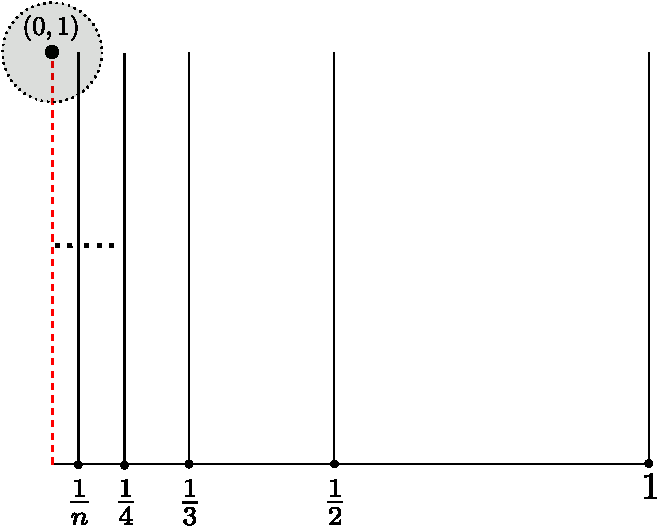
\includegraphics[scale=0.55]{Figuras/fig-pente}
\caption{O Pente Infinito}
\label{fig-pente}
\end{figure}

O ``pente infinito'' é um exemplo 
clássico de subconjunto conexo do plano que não é conexo por caminho.
O pente infinito é o subconjunto $\mathscr{P}$ do plano complexo, composto pelo ponto $(0,1)\in\mathbb{C}$
unido com os seguintes segmentos de reta: o segmento unindo o ponto $(0,0)$ ao ponto $(1,0)$ (base do pente);
e para cada $n\in\mathbb{N}$, o segmento unindo o ponto $(1/n,0)$ a $(1/n,1)$ (os ``dentes''do pente), 
veja a Figura \ref{fig-pente}.



A parte mais delicada de mostrar a conexidade do pente está relacionada 
a ideia intuitiva de que pente parece ter dois ``pedaços'': um contendo a ``base'' e os 
``dentes'' do pente; e outro contendo o ponto $(0,1)$. Isto porque não existe nenhum ``dente''
unindo o ponto $(0,0)$ da base do pente ao ponto $(0,1)$. 

Por outro lado, como sugere a figura acima, é impossível encontrar abertos disjuntos não-vazios
$U$ e $V$ tais que $\mathscr{P}\subset U\cup V$ e $(0,1)\in U$ e 
$\mathscr{P}\cap V\neq \emptyset$.
De fato, se existissem tais conjuntos existiria uma bola aberta centrada em $(0,1)$ 
com raio positivo, mas esta boa necessariamente interceptaria infinitos ``dentes'' 
evitando assim que o ponto $(0,1)$ e os demais pontos do pente possam ser separados
por abertos.

\medskip 

Vamos mostrar a seguir um resultado muito importante sobre a relação de conexidade e de 
conexidade por caminhos. Ele afirma que se $U\mathbb{C}$ é um 
conjunto aberto e conexo então 
quaisquer par de pontos em $U$ podem ser ligados por um caminho, suave por partes, inteiramente 
contido em $U$ e vice-versa. 

Alertamos o leitor menos experiente que a prova deste teorema pode ser omitida numa primeira
leitura e que as ideias envolvidas nela não são usadas no restante do texto.

\begin{teorema}\label{teo-conexo-conexo-caminhos}
Seja $U$ um subconjunto aberto  de $\mathbb{C}$. Então $U$ é conexo se, e somente se, 
$U$ é conexo por caminhos.
\end{teorema}

% \begin{proof}
% Vamos mostrar primeiro que se $U$ é um aberto conexo, então $U$ é conexo por caminhos. 
% De fato, primeiro para cada $z\in U$ seja $\mathscr{C}_{U}(z)$ o conjunto de todos os pontos
% $w\in U$ tais que $z$ e $w$ podem ser unidos por um caminho suave por partes inteiramente 
% contido em $U$, isto é, 
% \[
% \mathscr{C}_{U}(z) = 
% \left\{
% w\in U: 
% \begin{array}{l}
% \text{existe um caminho suave por partes}\ \gamma:[0,1]\to\mathbb{C}\\
% \text{tal que}\ \gamma([0,1])\subset U,\  \gamma(0)=z\ \text{e}\ \gamma(1)=w
% \end{array}
% \right\}.
% \] 
% Desta forma mostrar que $U$ é conexo por caminho se reduz a mostrar que 
% dado qualquer $z\in U$, então temos que $\mathscr{C}_{U}(z)=U$, uma vez que esta 
% igualdade significaria que se escolhemos qualquer ponto $w\in U$, então somos capazes 
% de encontrar um caminho, completamente contido em $U$, ligando $z$ a $w$. 

% Para mostrar que a igualdade acima é válida vamos mostrar primeiro que 
% para qualquer $z\in U$ dado que $\mathscr{C}_{U}(z)$ é um subconjunto aberto do plano complexo.
% Observe que independentemente da escolha de $z\in U$ o conjunto $\mathscr{C}_{U}(z)$ é não-vazio
% já que caminho constante liga $z$ a si mesmo. Continuando, para verificar 
% $\mathscr{C}_{U}(z)$ é aberto tomamos um ponto $w$ arbitrário em $\mathscr{C}_{U}(z)$.
% Como $\mathscr{C}_{U}(z)$ é sempre um subconjunto de $U$ então $w$ é um ponto de $U$, logo
% existe algum $r>0$ tal que $D(w,r)\subset U$. Vamos mostrar que todos os 
% pontos deste disco estão também contidos em $\mathscr{C}_{U}(z)$. 
% Feito isto podemos concluir que $w$ é um ponto interior de $\mathscr{C}_{U}(z)$. 
% Para mostrar isto basta observar que pela definição de 
% $\mathscr{C}_{U}(z)$ que existe algum caminho $\gamma_1:[0,1]\to\mathbb{C}$ totalmente contido em $U$
% unindo $z$ a $w$. Por outro lado, dado um ponto arbitrário $w' \in D(w,r)$ 
% temos que o caminho $\gamma_2:[1,2]\to\mathbb{C}$ dado por $\gamma_2(t)=w+(t-1)(w'-w)$,
% cuja curva associada é o segmento de reta unindo $w$ a $w'$ 
% é também um caminho totalmente contido em $D(w,r)\subset U$.
% Logo $\gamma_1*\gamma_2$ é um caminho suave por partes totalmente contido em $U$ unindo $z$ a $w'$.
% O que mostra que $w'\in \mathscr{C}_{U}(z)$. Como $w'$ foi escolhido arbitrariamente 
% em $D(w,r)$ temos que todo este disco está contido em $\mathscr{C}_{U}(z)$ o que implica que $w$
% é um ponto interior de $\mathscr{C}_{U}(z)$. Já que $w$ também foi escolhido arbitrariamente em 
% $\mathscr{C}_{U}(z)$ concluímos que este conjunto é aberto, pois todos seus pontos são pontos 
% interiores.

% Suponha, por absurdo, que 
% $V\equiv U\setminus \mathscr{C}_{U}(z)$ é um conjunto não-vazio.
% Seja $z'$ um ponto qualquer de $V$. Observe que $\mathscr{C}_{U}(z')$ 
% é disjunto de $\mathscr{C}_{U}(z)$, pois se existisse 
% um ponto $z''\in \mathscr{C}_{U}(z)\cap \mathscr{C}_{U}(z')$ 
% existiria um caminho $\gamma_1$ suave por partes totalmente contido em $U$ unindo
% $z$ a $z''$ e da mesma forma existiria um caminho $\gamma_2$ suave por partes 
% totalmente contido em $U$ unindo $z''$ a $z'$. Mas então $\gamma_1*\gamma_2$
% seria um caminho suave por partes totalmente contido em $U$ unindo $z$ a $z'$ 
% o que contraria a definição de $V$.
% Além de termos $\mathscr{C}_{U}(z)\cap \mathscr{C}_{U}(z')=\emptyset$ também temos que 
% \[
% V = \bigcup_{z'\in V} \mathscr{C}_{U}(z')
% \]
% é um conjunto aberto, já que ele é dado como uma união de conjuntos abertos. 
% Desta forma temos $U=\mathscr{C}_{U}(z)\cup V$ é uma união de dois abertos não-vazios 
% disjuntos o que é um absurdo, já que estamos assumindo que $U$ é conexo. 
% Esta contradição vem do fato de termos assumido 
% que $\mathscr{C}_{U}(z)\neq U$. Assim concluímos que todo aberto
% conexo de $\mathbb{C}$ é conexo por caminhos. 

% \medskip 
% Agora vamos provar a recíproca, isto é, se $U\subset \mathbb{C}$ é conexo 
% por caminhos então $U$ é conexo. 
% Para isto, seja $U$ um subconjunto de $\mathbb{C}$ conexo por caminhos.  
% Suponha, por absurdo, que $U=V_1\cup V_2$, onde $V_1$ e $V_2$ são 
% abertos não-vazios e disjuntos. Escolha arbitrariamente $z_1\in V_1$ e $z_2\in V_2$. 
% Por hipótese, existe algum caminho suave por partes $\gamma:[0,1]\to\mathbb{C}$ totalmente
% contido em $U$ unindo $z_1=\gamma(0)$ à $z_2=\gamma(1)$.
% Como $\gamma$ está totalmente contida em $U$ para todo $t\in [0,1]$ temos que
% $\gamma(t)\in V_1\cup V_2$. Já que $\gamma(0)=z_1$, $V_1$ e $V_2$ são abertos e $\gamma:[0,1]\to\mathbb{C}$
% é uma aplicação contínua então 
% o número 
% \[ 
% t^* \equiv \sup_{t\in [0,1]}\{ \gamma(t)\in V_1\}
% \]
% pertence ao intervalo aberto $(0,1)\subset\mathbb{R}$.
% Vamos mostrar a seguir que $\gamma(t^*)\in \partial V_2$.
% De fato, para qualquer $\varepsilon>0$ o disco $D(\gamma(t^*),\varepsilon)$
% intercepta $V_1$ e $V_1^c$ bem como $V_2$ e $V_2^c$. Para provar isto  usamos a continuidade de 
% $\gamma$ para verificar que para todo $\varepsilon>0$ existe $\delta>0$
% tal que se $|t-t^{*}|<\delta$ então $|\gamma(t)-\gamma(t^*)|<\varepsilon$. Em outras palavras
% para todo $t$ suficientemente próximo de $t^{*}$ temos $\gamma(t)\in D(\gamma(t^*),\varepsilon)$.
% Em seguida, observamos que pela definição de $t^*$ para qualquer $t$ fixado satisfazendo
% $t^{*}<t\leqslant 1$ temos $\gamma(t)\in V_2$. Se além desta condição impomos que 
% $|t-t^{*}|<\delta$ temos que este mesmo ponto $\gamma(t)\in D(\gamma(t^*),\varepsilon)$, pelas 
% escolhas de $\varepsilon$ e $\delta$. 
% Destas duas observações segue que a interseção $D(\gamma(t^*),\varepsilon)\cap V_2$
% é não-vazia. Por outro lado, como $t^{*}$ é o supremo dos $t$'s tais que $\gamma(t)\in V_1$
% sabemos que existe uma sequência $(t_n)_{n\in\mathbb{N}}$ tal que para todo $n\in\mathbb{N}$ 
% temos $0<t_n < t^*$, $t_n\to t^{*}$ e $\gamma(t_n)\in V_1$, para todo $n\in\mathbb{N}$.
% Pela definição de convergência de sequências existe $N_0\in\mathbb{N}$ tal que se $n\geqslant N_0$
% então $|t_n-t^{*}|<\delta$. Por esta última condição ser verdadeira segue que para qualquer $n\geqslant N_0$ temos
% $\gamma(t_n)\in D(\gamma(t^*),\varepsilon)$. Pela definição de $t_n$ temos que $\gamma(t_n)\in V_1$
% como $V_1$ e $V_2$ são disjuntos temos que $\gamma(t_n)\in V_2^c$ e portanto também é não vazia 
% a interseção $D(\gamma(t^*),\varepsilon)\cap V_2^c$. Destes argumentos podemos concluir que
% para todo $\varepsilon>0$ dado que 
% \[
% D(\gamma(t^*),\varepsilon)\cap V_2 \neq \emptyset 
% \qquad\text{e}\qquad
% D(\gamma(t^*),\varepsilon)\cap V_2^c \neq \emptyset.
% \]
% e finalmente que $\gamma(t^{*})\in \partial V_2$.
% Mas isto é um absurdo porque como $V_2$ é aberto sabemos que qualquer ponto de sua fronteira 
% está no seu complemento, mas como $\gamma$ está completamente contido em $U$ e também temos
% $U=V_1\cup V_2$ então segue que $\gamma(t^*)$ está necessariamente em $V_1$. Mas
% como $V_1$ é aberto existe algum $r>0$ tal que $D(\gamma(t^{*}),r)\subset V_1$.
% Tomando qualquer $\varepsilon>0$ tal que $\varepsilon<r$ concluiríamos que
% o disco $D(\gamma(t^{*}),\varepsilon)\subset D(\gamma(t^{*}),r)\subset V_1$
% mas como $D(\gamma(t^*),\varepsilon)\cap V_2 \neq \emptyset$ 
% então teríamos $V_1\cap V_2\neq\emptyset$ o que é um absurdo.

% \end{proof}


% \section{Limites e Continuidade de funções em $\mathbb{R}^2$}

% Nesta seção revisamos alguns conceitos básicos sobre limites e continuidade de funções 
% definidas em subconjuntos de $\mathbb{R}^2$ e tomando valores em $\mathbb{R}^2$. 
% Os conceitos topológicos considerados nesta seção são definidos de maneira
% análoga aos das seções anteriores usando a identificação natural
% de $\mathbb{C}$ com $\mathbb{R}^2$. 


% %Quando formos falar de distâncias nesta seção ao invés de usarmos a notação 
% %do módulo de $|z|$, onde $z=x+iy$ vamos usar a notação de norma do vetor $(x,y)$
% %isto é, $\|(x,y)\|=\sqrt{x^2+y^2}$, simplesmente para enfatizar que as ideias
% %discutidas não dependem da estrutura de produto de $\mathbb{C}$.


% Vamos nos restringir a aplicações definidas em conjuntos cujo o interior é não-vazio. 
% Para facilitar o leitor pode ter em mente conjuntos de $\mathbb{R}^2$ 
% correspondentes aos discos abertos de raio positivo ou 
% conjuntos como $D(z,r)\setminus\{z\}$ (o disco aberto de centro $z$ e raio $r$ exceto o ponto $z$).
% Como a estrutura de produto complexo não terá nenhuma relevância nesta seção vamos 
% conduzir as discussões usando a notação usual $(x,y)$ de vetores no plano. Já que esta
% seção tem caráter de revisão para
% manter semelhança com os textos de Cálculo em $\mathbb{R}^n$, vamos usar a linguagem 
% e notação de norma de vetor no lugar de falar do módulo de um número complexo. 

% O primeiro conceito que vamos recordar é o conceito de limite. 
% Seja $A\subset \mathbb{R}^2$ um conjunto de interior não-vazio. Vamos dizer que 
% um vetor $(a,b)\in\mathbb{R}^2$ é o limite de uma função 
% $f:A\subset \mathbb{R}^2\to\mathbb{R}^2$ quando $(x,y)\to (x_0,y_0)\in \overline{A}$
% se o vetor $f(x,y)$ fica arbitrariamente próximo do vetor $(a,b)$,  
% quando $(x,y)$ ficar arbitrariamente próximo de $(x_0,y_0)$. 
% Para denotar este fato usamos a notação 
% \[
% \lim_{(x,y)\to (x_0,y_0)} f(x,y) = (a,b).
% \]

% O problema com esta descrição intuitiva de limite  
% é que nela não temos um significa preciso do que é ``arbitrariamente próximo''. 
% Para remediar este problema vamos apresentar abaixo a definição formal de limite e 
% depois mostrar algumas outras formas equivalente dela.

% No que segue usamos a notação $\|\cdot\|$ para denotar a norma Euclidiana de um vetor
% em $\mathbb{R}^2$, isto é, 
% \[
% \|(x,y)\| = \sqrt{x^2+y^2}.
% \]



% \begin{definicao}\label{definicao-limite-R2}
% \index{Limite!de uma função}
% Seja $A\subset\mathbb{R}^2$ tal que interior de $A$ é não vazio e $f:A\to\mathbb{R}^2$ uma função.
% Dizemos que $f$ tem limite quando $(x,y)$ tende a $(x_0,y_0)\in \overline{A}$ (fecho de $A$) 
% se existe um vetor $(a,b)\in\mathbb{R}^2$ tal que para todo $\varepsilon>0$ dado existe um $\delta>0$
% tal que para todo ponto $(x,y)\in A$ satisfazendo $0<\|(x,y)-(x_0,y_0)\|<\delta$ 
% temos $\|f(x,y)-(a,b)\|<\varepsilon$. 
% Usamos a notação 
% \[
% \lim_{(x,y)\to (x_0,y_0)} f(x,y) = (a,b),
% \]
% para indicar que o ponto $(a,b)\in\mathbb{R}^2$ é o limite da função $f$ 
% quando $(x,y)$ tende a $(x_0,y_0)$. 
% \end{definicao}

% Uma observação importante a cerca desta definição é que não é necessário para falar de limite 
% que o ponto $(x_0,y_0)$ esteja no domínio da função $f$, isto é, não é necessário que a função $f$
% esteja definida no ponto $(x_0,y_0)$. Na verdade, basta que ela esteja definida em pontos suficientemente próximos
% deste ponto, o que de maneira mais precisa significa dizer que $(x_0,y_0)$ é um ponto do fecho do domínio de $f$
% que poderia não estar no domínio da função $f$. Este é inclusive um dos casos mais interessantes quando estamos 
% falando de limites. 


% Lembramos que cada função $f:A\subset\mathbb{R}^2\to\mathbb{R}^2$ é determinada por suas funções coordenadas, 
% isto é, existem funções reais $u:A\subset\mathbb{R}^2\to\mathbb{R}$ e 
% $v:A\subset\mathbb{R}^2\to\mathbb{R}$ tais que
% para todo $(x,y)\in A$ temos $f(x,y)=(u(x,y),v(x,y))$.
% Além do mais podemos verificar que existe o limite 
% \[
% \lim_{(x,y)\to (x_0,y_0)} f(x,y) = (a,b),
% \]
% se e somente se,
% \[
% \lim_{(x,y)\to (x_0,y_0)} u(x,y) = a
% \qquad \text{e} \qquad 
% \lim_{(x,y)\to (x_0,y_0)} v(x,y) = b,
% \]
% onde a definição destes limites acima são feitas de maneira análoga à 
% Definição \ref{definicao-limite-R2}, mas substituindo onde aparece $\|f(x,y)-(a,b)\|<\varepsilon$
% por $|u(x,y)-a|<\varepsilon$ e $|v(x,y)-b|<\varepsilon$, respectivamente. 


% Uma função $f$ pode ter limite quando $(x,y)$ tende a um ponto $(x_0,y_0)$, o ponto 
% $(x_0,y_0)$ pode ser um ponto do domínio de $f$, mas a imagem do ponto $(x_0,y_0)$ pela 
% função $f$ pode não coincidir com este limite. Este é o caso do seguinte exemplo.

% Seja $f:\mathbb{R}^2\to\mathbb{R}^2$ a função dada por
% \[
% f(x,y)
% =
% \begin{cases}
% (0,0),&\text{se}\ (x,y)\neq (0,0);
% \\
% (0,1),&\text{se}\ (x,y)=(0,0).
% \end{cases}
% \]
% Então podemos verificar que 
% \[
% \lim_{(x,y)\to (0,0)}f(x,y) = (0,0), 
% \quad\text{porém}\quad 
% \lim_{(x,y)\to (0,0)}f(x,y) \neq  f(0,0). 
% \]

% Funções que, ao contrário destas do exemplo, têm a propriedade de que 
% para qualquer ponto de seu domínio $(x_0,y_0)$ temos
% \[
% \lim_{(x,y)\to (x_0,y_0)}f(x,y) =  f(x_0,y_0) 
% \]
% são chamadas de funções contínuas. Tais funções possuem uma série de propriedades muito 
% especiais e formam um classe de funções razoavelmente grande, 
% onde uma teoria rica de resultados 
% interessantes pode ser desenvolvida.

% \begin{definicao}\label{func-cont-plano}
% \index{Função!contínua}
% Sejam $A\subset \mathbb{R}^2$ um aberto e $f:A\to\mathbb{R}^2$ uma função.
% Dizemos que $f$ é contínua em um ponto $(x_0,y_0)\in A$ se 
% \[
% \lim_{(x,y)\to (x_0,y_0)}f(x,y) =  f(x_0,y_0).
% \]
% Se $f$ é contínua em todos os pontos de $A$, dizemos que $f$ é contínua em $A$.
% \end{definicao}

% A continuidade de um certo ponto de vista é uma propriedade de regularidade muito importante.
% Outra classe de funções com propriedades muito interessantes também é a classe das funções 
% que admitem derivadas parciais.

% \begin{definicao}\label{def-deriv-parciais}
% \index{Derivadas!parciais}
% Sejam $A\subset \mathbb{R}^2$ um aberto e $f:A\to\mathbb{R}^2$ uma função.
% Dizemos que $f$ tem derivada parcial em relação a $x$ no ponto $(x_0,y_0)\in A$
% se existe o seguinte limite
% \[
% \lim_{h\to 0} \frac{f(x_0+h,y_0)-f(x_0,y_0)}{h},
% \]
% Analogamente, $f$ tem derivada parcial em relação a $y$ no ponto $(x_0,y_0)\in A$
% se existe o seguinte limite 
% \[
% \lim_{k\to 0} \frac{f(x_0,y_0+k)-f(x_0,y_0)}{h}.
% \]
% \end{definicao}
% Caso existam as derivadas parciais em relação a $x$ e $y$
% elas são denotadas por, respectivamente, por
% \[
% \frac{\partial }{\partial x}f(x_0,y_0)
% \quad \text{e}\quad
% \frac{\partial }{\partial y}f(x_0,y_0).
% \]
% Observamos que estas duas derivadas parciais são vetores em $\mathbb{R}^2$.
% Se $u$ e $v$ são as coordenadas de $f$ então as derivadas parciais acima são dadas por
% \[
% \frac{\partial }{\partial x}f(x_0,y_0)
% =
% \left(\frac{\partial }{\partial x}u(x_0,y_0), \frac{\partial }{\partial x}v(x_0,y_0)  \right)
% \]
% e
% \[
% \frac{\partial}{\partial y}f(x_0,y_0)
% =
% \left(\frac{\partial}{\partial y}u(x_0,y_0), \frac{\partial}{\partial y}v(x_0,y_0)  \right).
% \]

% Se as derivadas parciais de $f$ em relação a $x$ e$y$ existem em todos os pontos de $A$,
% podemos definir duas novas funções definidas em $A$ e tomando em $\mathbb{R}^2$ como segue:
% \[
% (x,y)\longmapsto \frac{\partial}{\partial x}f(x,y)
% \quad \text{e}\quad 
% (x,y)\longmapsto \frac{\partial}{\partial y}f(x,y).
% \]
% Caso estas aplicações sejam contínuas em $A$, vamos dizer que $f$ é uma aplicação 
% de classe $C^1$ em $A$. Note que a função $f=(u,v)$ é de classe $C^1$ em $A$ 
% se, e somente se, as seguintes funções 
% \[
% \frac{\partial}{\partial x}u(x,y),
% \quad
% \frac{\partial}{\partial y}u(x,y),
% \quad 
% \frac{\partial}{\partial x}v(x,y)
% \ \text{e}\quad 
% \frac{\partial}{\partial y}v(x,y)
% \]
% são contínuas em $A$.

% \begin{exemplo} A função $f:\mathbb{R}^2\setminus\{(0,0)\}$ dada por 
% \[
% f(x,y)
% =
% \left( \frac{-y}{x^2+y^2}, \frac{x}{x^2+y^2} \right)
% \]
% é uma função de classe $C^1$ em $A$, já que suas derivadas parciais são dadas por 
% \[
% \frac{\partial}{\partial x}f(x,y)
% =
% \left( \frac{2xy}{(x^2+y^2)^2}, \frac{y^2-x^2}{(x^2+y^2)^2}  \right)
% \]
% e
% \[
% \frac{\partial}{\partial x}f(x,y)
% =
% \left( \frac{y^2-x^2}{(x^2+y^2)^2}, \frac{-2xy}{(x^2+y^2)^2}  \right).
% \]
% \end{exemplo}


% \section{Integrais de Linha e o Teorema de Green}

% Nesta seção vamos recordar um dos resultados mais importante sobre integrais de linha 
% em $\mathbb{R}^2$ que é o Teorema de Green. As integrais de linha serão usadas para
% desenvolvermos a teoria de integração no plano complexo. Embora a integral complexa não seja 
% exatamente igual a integral de linha, que será definida a seguir, elas se relacionam. 
% É importante explorar estas relações para podermos aplicar o Teorema de Green 
% para provar um dos resultados mais importantes sobre integração complexa, 
% que serão discutidos neste texto. Por esta razão vamos dedicar esta seção ao 
% Teorema de Green. 

% Esta seção está organizada da seguinte maneira. Primeiro recordamos algumas 
% definições e conceitos básicos e em seguida apresentamos uma prova elementar 
% do Teorema de Green, válida em situações bastante gerais. 


% \bigskip 


% Para simplificar os enunciados das definições e teoremas desta seção, 
% vamos assumir que daqui por diante 
% $A\subset\mathbb{R}^2$ sempre denotará um domínio (aberto e conexo) e
% que $f:A\to\mathbb{R}^2$ é 
% uma função de classe $C^1$ em $A$ e dada em coordenadas por $f(x,y)=(u(x,y),v(x,y))$.

% \begin{definicao}[Integral de Linha]
% \label{def-int-linha-R2}
% \index{Integral!de linha em $\mathbb{R}^2$}
% Seja $\gamma:[a,b]\to\mathbb{C}$ um caminho suave inteiramente contido em $A$. 
% Definimos a integral de $f$ ao longo de $\gamma$
% (ou integral de linha de $f$ ao longo de $\gamma$) pela seguinte expressão
% \[
% \int_{\gamma} f 
% \equiv
% \int_{a}^{b} \langle f\circ\gamma(t),\gamma'(t) \rangle \, dt,
% \]
% onde $\langle\cdot,\cdot\rangle$ denota o produto interno canônico de $\mathbb{R}^2$.
% \end{definicao}

% Apresentamos a definição de integral de linha sem especificá-la a partir de coordenadas
% por motivos de comparação com a integral complexa que será introduzida mais a frente.

% De qualquer forma é muito importante ter em mente como se escreve esta integral em coordenadas.
% Portanto, se $\gamma(t)=(x(t),y(t))$ então temos  
% \begin{align}\label{eq1-forma-dif-int-linha}
% \int_{\gamma} f 
% &\equiv
% \int_{a}^{b} \langle f\circ\gamma(t),\gamma'(t) \rangle \, dt
% \nonumber \\
% &=
% \int_{a}^{b} u(x(t),y(t))x'(t) \, dt + \int_{a}^{b} v(x(t),y(t))y'(t) \, dt.
% \end{align}
% Note que esta identidade também revela que a integral de $f$ ao longo de $\gamma$ está bem definida
% para classe de funções e caminhos que estamos considerando neste texto já que 
% as funções $u,v,x'$ e $y'$ são funções contínuas
% e $[a,b]$ é um intervalo de comprimento finito da reta.


% Esta identidade também sugere a introdução da seguinte notação alternativa para integral 
% de linha de $f$ ao longo de $\gamma$
% \begin{align}\label{eq2-forma-dif-int-linha}
% \int_{\gamma} f
% \equiv 
% \int_{\gamma} u\, dx + \int_{\gamma} v \, dy,
% \end{align}
% onde o significado preciso das primeira e segunda parcelas do lado direito acima 
% são dados pelas parcelas que aparecem em \eqref{eq1-forma-dif-int-linha},
% respectivamente.

% %Mas de qualquer forma é importante também recordar como calcular uma integral de linha 
% %em casos concretos onde conhecemos as coordenadas do caminho $\gamma$ bem como da função $f$.
% %
% %Observamos que se para cada $t\in [a,b]$ o caminho suave $\gamma$ é dado
% %em coordenadas por $\gamma(t)=(x(t),y(t))$ então temos:
% %\begin{align*}
% %\int_{\gamma} f 
% %&=
% %\int_{a}^{b} \langle f\circ\gamma(t),\gamma'(t) \rangle \, dt,
% %\\[0.3cm]
% %&=
% %\int_{a}^{b} \Big\langle \big(u(x(t),y(t)),v((x(t),y(t))\big), \big(x'(t),y'(t)\big) \Big\rangle\, dt
% %\\
% %&=
% %\int_{a}^{b} u(x(t),y(t))x'(t)+ v((x(t),y(t))y'(t)\, dt.
% %\end{align*}


% Observamos  que a definição estende-se naturalmente para o caso de caminhos suaves por partes.
% Mais precisamente, se $\gamma_1*\ldots*\gamma_n$ é um caminho suave por partes em $A$, 
% então definimos a integral de linha de $f$ ao longo de $\gamma$ pela seguinte expressão
% \[
% \int_{\gamma_1*\ldots*\gamma_n} f
% \equiv 
% \int_{\gamma_1}f +\ldots+\int_{\gamma_n}f.
% \]

% Em geral, é mais prático adotar notações um pouco mais curtas para denotar a integral de linha 
% acima. Por exemplo, para simplificar a expressão no lado esquerdo 
% da definição acima. chamamos de $\gamma$ o caminho suave por partes $\gamma_1*\ldots*\gamma_n$. 
% Quanto ao lado direito podemos usar a notação de somatório. Desta 
% forma a definição pode ser reescrita em uma notação mais condensada como segue
% \[
% \int_{\gamma} = \sum_{j=1}^n \int_{\gamma_j}f\, .
% \]


% \begin{exemplo}
% Seja $A=\mathbb{R}^2\setminus\{(0,0)\}$ e $f:A\to\mathbb{R}^2$ dada por 
% \[
% f(x,y) = \left( \frac{-y}{x^2+y^2},\frac{x}{x^2+y^2} \right).
% \]
% Então a integral de $f$ ao longo do caminho suave $\gamma:[0,2\pi]\to \mathbb{C}$
% definido em coordenadas por $\gamma(t)=(\cos t,\sen t)$ é dada por 
% \begin{align*}
% \int_{\gamma} f
% &=
% \int_{0}^{2\pi} \langle f\circ\gamma(t),\gamma'(t) \rangle \, dt
% \\[0.3cm]
% &=
% \int_{0}^{2\pi} 
% 	\left\langle 
% 		\left( \frac{-\sen t}{\sen^2 t+\cos^2 t}  , \frac{\cos t}{\sen^2 t+\cos^2 t} \right)
% 		\ , \ 
% 		(-\sen t,\cos t)    
% 	\right\rangle 
% 	dt
% \\[0.3cm]
% &=
% \int_{0}^{2\pi} \sen^2 t+\cos^2 t \  dt
% =
% 2\pi.
% \end{align*}
% \end{exemplo}


% \begin{exemplo}\label{exemplo-z2-em-R2}
% Neste exemplo consideramos $A=\mathbb{R}^2$ e $\gamma_1*\gamma_2*\gamma_3^{-}*\gamma_4^{-}$ 
% o caminho suave por partes, onde 
% \begin{align*}
% \gamma_1(t) = (0,t),\ 0\leqslant t\leqslant 1;
% \\[0.2cm]
% \gamma_2(t) = (t,1),\ 0\leqslant t\leqslant 1;
% \\[0.2cm]
% \gamma_3(t) = (1,t),\ 0\leqslant t\leqslant 1;
% \\[0.2cm]
% \gamma_4(t) = (t,0),\ 0\leqslant t\leqslant 1.
% \end{align*}
% Note que a curva associada a $\gamma_1*\gamma_2*\gamma_3^{-}*\gamma_4^{-}$  
% é justamente $\partial ([0,1]\times[0,1])$ orientado no sentido horário.

% Seja $f:\mathbb{R}^2\to\mathbb{R}^2$ dada por $f(x,y)=(x^2-y^2,2xy)$. Então a integral 
% de linha de $f$ ao longo de $\gamma_1*\gamma_2*\gamma_3^{-}*\gamma_4^{-}$ é dada por

% \begin{align*}
% \int_{\gamma_1*\gamma_2*\gamma_3^{-}*\gamma_4^{-}} f
% &=
% \int_{0}^{1} \langle f\circ\gamma_1(t),\gamma_1'(t) \rangle \, dt
% +
% \int_{0}^{1} \langle f\circ\gamma_2(t),\gamma_2'(t) \rangle \, dt
% \\
% &\quad +
% \int_{0}^{1} \langle f\circ\gamma^{-}_3(t),(\gamma^{-}_3)'(t) \rangle \, dt
% +
% \int_{0}^{1} \langle f\circ\gamma^{-}_4(t),(\gamma^{-}_4)'(t) \rangle \, dt.
% \end{align*}

% Observe que
% \[ 
% \begin{array}{lll}
% \gamma_1(t) = (0,t), 		& \qquad f\circ\gamma_1(t)=(-t^2,0),			& \qquad \gamma_{1}'(t)=(0,1) 
% \\[0.2cm]
% \gamma_2(t) = (t,1), 		& \qquad f \circ\gamma_2(t)=(t^2-1,2t),			& \qquad\gamma_{2}'(t)=(1,0) 
% \\[0.2cm]
% \gamma^{-}_3(t) = (1,1-t), 	& \qquad f \circ\gamma^{-}_3(t)=(2t-t^2,2-2t),& \qquad(\gamma_{3}^{-})'(t)=(0,-1) 
% \\[0.2cm]
% \gamma^{-}_4(t) = (1-t,0), 	& \qquad f\circ\gamma^{-}_4(t)=(1-2t+t^2,0), 	& \qquad(\gamma_{4}^{-})'(t)=(-1,0).
% \end{array}
% \]
% Portanto 
% \begin{align*}
% \int_{\gamma_1*\gamma_2*\gamma_3^{-}*\gamma_4^{-}} f
% &=
% \int_{0}^{1} (t^2-1)\, dt
% +
% \int_{0}^{1} (2t-2)\,  dt
% +
% \int_{0}^{1} (-t^2+2t-1)\, dt
% \\[0.2cm]
% &
% =
% 4\int_{0}^{1}t\, dt -4
% \\[0.2cm]
% &= 
% -2.
% \end{align*}
% \end{exemplo}


% Lembramos que as integrais de linha são sensíveis a orientação do caminho de forma
% que se invertemos a orientação do caminho então mudamos o sinal da integral, como mostrado abaixo
% \[
% \int_{\gamma^{-}} f = -\int_{\gamma} f.
% \]
% Esta relação pode ser facilmente deduzida da fórmula de mudança de variáveis para integrais
% como segue. Seja $\gamma:[a,b]\to\mathbb{R}^2$ um caminho suave. Como já vimos anteriormente
% $\gamma^{-}:[a,b]\to\mathbb{R}^2$ é dado por $\gamma\circ r(t)$, onde $r(t)=a+b-t$.
% \begin{align}\label{eq-int-linha-gamma-reverso}
% \int_{\gamma^{-}}f
% &=
% \int_{a}^{b} \langle f\circ\gamma^{-}(t),(\gamma^{-})'(t) \rangle \, dt
% \nonumber
% \\
% &=
% \int_{a}^{b} \langle (f\circ\gamma\circ r)(t),\frac{d}{dt}(\gamma\circ r)(t) \rangle \, dt
% \nonumber
% \\
% &=
% \int_{a}^{b} \langle f(\gamma(r(t))),\gamma'(r(t))r'(t) \rangle \, dt
% \nonumber
% \\
% &=
% \int_{a}^{b} \langle f(\gamma(r(t))),\gamma'(r(t))\rangle r'(t)\, dt.
% \end{align}
% Lembramos agora a fórmula de mudança de variáveis. Se $g:\mathbb{R}\to\mathbb{R}$ é uma função
% contínua e $r:\mathbb{R}\to\mathbb{R}$ é uma função derivável. Então 
% \[
% \int_{a}^{b} g(r(t))r'(t)\, dt = \int_{r(a)}^{r(b)} g(t)\, dt.
% \]
% Tomando $g(t)= \langle f(\gamma(t)),\gamma'(t)\rangle$ e aplicando a fórmula de mudanças
% de varíaveis no lado direito de \eqref{eq-int-linha-gamma-reverso} ficamos com
% \begin{align*}
% \int_{a}^{b} \langle f(\gamma(r(t))),\gamma'(r(t))\rangle r'(t)\, dt
% &=
% \int_{a}^{b} g(r(t))r'(t)\, dt
% \\[0.2cm]
% &=
% \int_{r(a)}^{r(b)} g(t)\, dt
% \\[0.2cm]
% &=
% \int_{b}^{a} \langle f(\gamma(t)),\gamma'(t)\rangle\, dt
% \\[0.2cm]
% &=
% -\int_{a}^{b} \langle f(\gamma(t)),\gamma'(t)\rangle\, dt
% \\[0.2cm]
% &=
% -\int_{\gamma} f.
% \end{align*}


% Antes de enunciarmos o Teorema de Green vamos lembrar a definição de compatibilidade 
% entre uma região e sua fronteira. 

% \begin{definicao}
% 	\index{Orientação!compatível}
% 	Suponha que $U\subset \mathbb{R}^2$ é um domínio e seja 
% 	$V\subset U$ um subconjunto compacto, cuja fronteira consiste de um 
% 	número finito de curvas de Jordan suaves por partes e tal que 
% 	$V\setminus \partial V$ é um domínio. Para cada uma dessas curvas,
% 	adotamos  o sentido de percurso para o qual o interior de $V$ está sempre 
% 	à esquerda quando a percorremos. Nestas condições dizemos que $V$ 
% 	e $\partial V$ têm sentido compatível.
% \end{definicao}

% Esta noção será empregada diversas vezes ao longo do texto e recomendamos que o leitor a tenha em mente.

% \begin{exemplo}
% Seja $U=\mathbb{R}^2$ e $V=D(0,r)$, cuja a fronteira é o conjunto $\partial V= \partial D(0,r)$. 
% Para que $V$ e $\partial V$ tenham orientação compatível $\partial V$ deve ser percorrida
% no sentido anti-horário como mostra a figura abaixo.
% \end{exemplo}


% \begin{exemplo}
% Neste exemplo tomamo novamente $U=\mathbb{R}^2$ e $V$ como 
% mostrado na figura abaixo. Para que $\partial V = \gamma_1*\gamma_2*\gamma_3$
% tenham orientação compatível com $V$ estas curvas devem ser percorridas como 
% mostrado no figura, isto é, $\gamma_1$ no sentido anti-horário; e $\gamma_2$ e $\gamma_3$
% no sentido horário.
% \end{exemplo}


% \begin{teorema}[Teorema de Green]
% \label{teo-Green}
% \index{Teorema! de Green}
% Sejam $U\subset \mathbb{R}^2$ um domínio e $f:U\to\mathbb{R}^2$ uma aplicação 
% de classe $C^1$. Seja $V\subset U$ um subconjunto satisfazendo
% \begin{itemize}
% 	\item $V$ é compacto;
% 	\item $\partial V = \gamma_1*\ldots*\gamma_n$ é formada por uma quantidade finita de curvas de 
% 	Jordan suaves por partes;
% 	\item $V\setminus\partial V$ é um domínio; 
% \end{itemize}
% Suponha que $V$ e $\partial V$ têm orientação compatível e que $f$ em coordenadas é 
% escrita como $f(x,y)=(u(x,y),v(x,y))$, então 
% \[
% \int_{\partial V} f = \iint_{V} \left(  \frac{\partial}{\partial x}v(x,y)- \frac{\partial}{\partial y}u(x,y) \right) \, dxdy.
% \]
% \end{teorema}


% \begin{proof}
% A prova deste teorema como enunciada exige ferramental mais sofisticado do que temos disponível neste momento.
% Entretanto podemos apresentar uma prova simples e ilustrativa para o caso em que o conjunto $V$ 
% pode ser descrito como uma região que é simultaneamente verticalmente e horizontalmente simples, ou seja,
% \begin{align*}
% V=
% \left\{ 
% 	(x,y)\in \mathbb{R}^2 : a\leqslant x\leqslant b, \
% 	\begin{array}{l}
% 		g_1(x)\leqslant y\leqslant g_2(x),\ \text{onde}\ g_1 \text{e}\ g_2 \ \text{são funções}
% 		\\
% 		\text{cujos gráficos são curvas suaves por partes} 
% 	\end{array}
% \right\}
% \end{align*}
% e 
% \begin{align*}
% V=
% \left\{ 
% 	(x,y)\in \mathbb{R}^2 : c\leqslant y\leqslant d, \
% 	\begin{array}{l}
% 		h_1(x)\leqslant x\leqslant h_2(x),\ \text{onde}\ h_1 \text{e}\ h_2 \ \text{são funções}
% 		\\
% 		\text{cujos gráficos são curvas suaves por partes} 
% 	\end{array}
% \right\},
% \end{align*}
% respectivamente.

% Lembrando \eqref{eq2-forma-dif-int-linha} podemos decompor a integral de linha de $f$ ao longo de $\partial V$
% como segue
% \[
% \int_{\partial V} f = \int_{\partial V} u\, dx +\int_{\partial V} v\, dy.
% \]
% A estratégia para provar o Teorema de Green  
% será primeiramente olhar para $V$ como um conjunto verticalmente simples 
% e deduzir a seguinte igualdade
% \begin{align}\label{eq-conclusao1-teo-green}
% \int_{\partial V} u\, dx = -\iint_{V} \frac{\partial}{\partial y}u(x,y)\, dxdy.
% \end{align}
% Em seguida, olhamos  para $V$ como um conjunto horizontalmente simples e mostramos
% que 
% \begin{align}\label{eq-conclusao2-teo-green}
% \int_{\partial V} v\, dy = \iint_{V} \frac{\partial}{\partial x}v(x,y)\, dxdy.
% \end{align}
% Após obtidas as duas igualdades acima basta somá-las para finalizar a prova.

% \bigskip 

% Para executar a primeira parte da nossa estratégia vamos olhar para $V$ como uma região 
% verticalmente simples. Para escrever sua fronteira como um caminho suave por partes consideramos
% os seguinte caminhos suaves:
% \[
% \begin{array}{lc}
% \gamma_1(t) = (t,g_1(t)),& a\leqslant t\leqslant b;
% \\
% \gamma_2(t) = (b,t),& g_1(b)\leqslant t\leqslant g_2(b);
% \\
% \gamma_{3}(t) = (t,g_2(t)),&  a\leqslant t\leqslant b;
% \\
% \gamma_{4}(t) = (a,t),& g_1(b)\leqslant t\leqslant g_2(b);
% \end{array} 
% \]

% Para que a região $V$ e sua fronteira tenham orientação compatível devemos ter 
% $\partial V  = \gamma_1*\gamma_2*\gamma^{-}_3*\gamma^{-}_4$ e portanto 
% \[
% \int_{\partial V} u \, dx
% =
% \int_{\gamma_1} u\, dx
% +
% \int_{\gamma_2} u\, dx
% +
% \int_{\gamma^{-}_3} u\, dx
% +
% \int_{\gamma^{-}_4} u\, dx.
% \]
% Já que $\gamma_2'(t)=(0,1)$ e $(\gamma_4^{-})'(t)=(0,-1)$ a segunda e quarta integrais,
% do lado direito da igualdade, acima são nulas. Assim ficamos com 
% \begin{align}\label{eq-aux1-teo-green}
% \int_{\partial V} u \, dx
% &=
% \int_{\gamma_1} u\, dx
% +
% \int_{\gamma^{-}_3} u\, dx
% \nonumber
% \\
% &=
% \int_{a}^{b} u(t,g_1(t))\, dt -\int_{a}^{b} u(t,g_2(t))\, dt
% \nonumber
% \\
% &=
% \int_{a}^{b} [u(t,g_1(t))-u(t,g_2(t))]\, dt.
% \end{align}

% Observe que para cada $t$ fixado entre $a$ e $b$ podemos usar o teorema fundamental do cálculo
% para representar 
% \[
% u(t,g_1(t))-u(t,g_2(t)) 
% =
% \int_{g_2(t)}^{g_1(t)} \frac{\partial}{\partial y}u(t,y)\, dy
% =
% -\int_{g_1(t)}^{g_2(t)} \frac{\partial}{\partial y}u(t,y)\, dy
% \]
% Substituindo esta expressão no lado direito de \eqref{eq-aux1-teo-green}
% e usando o Teorema de Fubini (que afirma que a integral dupla coincide com a integral iterada)
% ficamos com 
% \begin{align*}
% \int_{\partial V} u \, dx
% &=
% \int_{a}^{b} [u(t,g_1(t))-u(t,g_2(t))]\, dt
% \\[0.3cm]
% &=
% -\int_{a}^{b} \int_{g_1(t)}^{g_2(t)} \frac{\partial}{\partial y}u(t,y)\, dy dt
% \\[0.3cm]
% &=
% -\iint_{V} \frac{\partial }{\partial y}u(x,y) \, dxdy,
% \end{align*}
% o que encerra a prova de \eqref{eq-conclusao1-teo-green}.

% Passamos agora para a prova de \eqref{eq-conclusao2-teo-green}. Agora vamos olhar para $V$ como 
% uma região horizontalmente simples. Neste caso sua fronteira poderá ser descrita por meio das seguintes
% curvas suaves
% \[
% \begin{array}{lc}
% 	\gamma_1(t) = (t,c),& h_1(c)\leqslant t\leqslant h_2(c);
% 	\\[0.2cm]
% 	\gamma_2(t) = (h_2(t),t),& c\leqslant t\leqslant d;
% 	\\[0.2cm]
% 	\gamma_{3}(t) = (t,d),&  h_1(d)\leqslant t\leqslant h_2(d);
% 	\\[0.2cm]
% 	\gamma_{4}(t) = (h_1(t),t),& c\leqslant t\leqslant d;
% \end{array} 
% \]
% Agora
% \[
% \int_{\partial V} v\, dy
% =
% \int_{\gamma_1} v\, dy
% +
% \int_{\gamma_2} v\, dy
% +
% \int_{\gamma^{-}_3} v\, dy
% +
% \int_{\gamma^{-}_4} v\, dy.
% \]
% Já que $\gamma_1'(t)=(1,0)$ e $(\gamma^{-}_3)'(t)=(-1,0)$ podemos verificar que a primeira e terceira integrais no 
% lado direito da igualdade acima são nulas e que a seguinte igualdade é válida
% \begin{align*}
% \int_{\partial V} v\, dy
% &=
% \int_{\gamma_2} v\, dy
% +
% \int_{\gamma^{-}_4} v\, dy.	
% \\
% &=
% \int_{c}^{d} v(h_2(t),t)\, dt -\int_{c}^{d} v(h_1(t),t)\, dt
% \\
% &=
% \int_{c}^{d} [v(h_2(t),t) -  v(h_1(t),t)]\, dt.
% \end{align*}
% Analogamente ao caso anterior, para qualquer $t$ fixado entre $c$ e $d$ podemos aplicar o Teorema Fundamental 
% do Cálculo para representar 
% \[
% v(h_2(t),t) -  v(h_1(t),t) = \int_{h_1(t)}^{h_2(t)} \frac{\partial}{\partial x}v(x,t)\, dx.
% \]
% Substituindo a expressão acima no lado direito da igualdade anterior e em seguida
% aplicando novamente o Teorema de Fubini concluímos que 
% \[
% \int_{\partial V} v\, dy
% =
% \int_{c}^{d}  \int_{h_1(t)}^{h_2(t)} \frac{\partial}{\partial x}v(x,t)\, dx dt
% =
% \iint_{V} \frac{\partial}{\partial x}v(x,y)\, dx dy,
% \]
% o que prova \eqref{eq-conclusao2-teo-green}. Somando \eqref{eq-conclusao1-teo-green} e 
% \eqref{eq-conclusao2-teo-green} membro-a-membro encerramos finalmente 
% a prova do Teorema de Green.
% \end{proof}



% \begin{exemplo}
% Vamos usar o Teorema do Green para re-obter o resultado calculado no Exemplo \ref{exemplo-z2-em-R2}.
% Naquele exemplo a função $f$ estava definida em todo $\mathbb{R}^2$ que na terminologia do nosso enunciado
% do Teorema de Green corresponde ao domínio $U$. Observe também que a função $f$ daquele exemplo
% é de classe $C^1$.  Agora, o compacto $V$ do enunciado do Teorema de Green 
% é o conjunto  $V=[0,1]\times[0,1]$. Como sabemos sua fronteira é composta por quatro caminhos suaves.
% É claro que $V\setminus\partial V$ é um domínio. Um outro detalhe importante é que
% a integral de $f$ ao longo da fronteira de $V$ no Exemplo \ref{exemplo-z2-em-R2} 
% considerava $\partial V$ orientada no sentido horário. 
% Mas note que com esta orientação $V$ e $\partial V$ não estão compativelmente orientados. 
% Logo  para aplicar o Teorema de Green precisamos mudar a orientação de $\partial V$ considerada naquele exemplo.
% Então para re-obter o valor da integral de linha daquele exemplo, basta 
% aplicar o Teorema de Green e depois mudar o  sinal do resultado obtido aqui.

% Lembramos que $f(x,y)=(u(x,y),v(x,y))=(x^2-y^2,2xy)$ e portanto 
% \[
% -\frac{\partial }{\partial y}u(x,y) = -\frac{\partial}{\partial y}(x^2-y^2)= -2y
% \qquad\text{e}\qquad
% \frac{\partial}{\partial x}v(x,y) = \frac{\partial}{\partial x}2xy = 2y.
% \]
% Considerando $\partial V$ orientado no sentido anti-horário temos pelo Teorema de 
% Green que 
% \[
% \int_{\partial V} f = \iint_{[0,1]\times[0,1]} 2y-(-2y)\, dxdy = \int_{0}^{1}\int_{0}^{1} 4y \, dxdy = \int_{0}^{1}4y\, dy =2.
% \]

% \end{exemplo}




%\begin{subappendices}
%\markboth{Ap\^{e}ndice 1}{Ap\^{e}ndice 1}

% Neste apêndice relacionamos alguns tópicos e resultados que não são normalmente apresentados
% em um curso introdutório de cálculo em uma variável complexa. Em geral, os tópicos tratados
% aqui costumam ser discutido em detalhes e mais profundidade em quaisquer bons livros de 
% Análise Real e Complexa. Ao leitor interessado recomendamos a referência \cite{MR3331079}.

% \section{Supremo e Ínfimo de Subconjuntos da Reta}\label{Apend-sup-inf}

% Um conjunto $B\subset \mathbb{R}$ é dito limitado superiormente, se existe um número $c\in\mathbb{R}$
% tal que $b\leqslant c$ para todo $b\in B$. O número $c$ é chamado de uma {\bf cota superior} 
% de $B$. 
% Analogamente, um conjunto $B$ é dito limitado inferiormente, se existe um número $a\in\mathbb{R}$ 
% tal que $a\leqslant b$ para todo $b\in B$. Neste caso o número $a$ é chamado de cota inferior
% de $B$.

% \begin{definicao}[Supremo]\label{def-sup}\index{Supremo}
% Dizemos que um número real $s$ é a menor cota superior de um conjunto $B$ limitado superiormente se satisfaz as seguintes condições:
% \begin{enumerate}[i)]
% \item $s$ é uma cota superior de $B$; 
% \item  se $s'$ é qualquer outra cota superior de $B$ então $s\leq s'$. 
% \end{enumerate}
% O número $s$ que é menor cota superior de um conjunto $B$ é denotado 
% por $\sup(B)$ e chamado de supremo do conjunto $B$.
% \end{definicao}
% Quando o conjunto $B$ não é limitado superiormente, ele não possui nenhuma cota superior e nestes casos definimos $\sup(B)=+\infty$.

% O conjunto dos números reais goza da seguinte propriedade: qualquer subconjunto limitado de $\mathbb{R}$
% possui um supremo. 

% Na seção anterior nós trabalhamos com supremo. Lá o conjunto $B$ era um 
% conjunto de números reais da forma 
% $B= \{|w-z|\in\mathbb{R} : w,z\in U\}$ para algum $U\subset \mathbb{C}$.

% O conceito de supremo generaliza o conceito de máximo. Por exemplo,
% se $B$ é um conjunto finito digamos $B=\{b_1,b_2,\ldots,b_n\}$ podemos sempre
% encontrar pelo menos um índice $j\in \{1,\ldots,n\}$ tal que $b_i\leqslant b_j$
% para todo $i\in\{1,\ldots,n\}$. Neste caso o elemento $b_j$ é chamado de máximo de $B$,
% e denotado por $b_j=\max\{b_1,\ldots,b_j\}$.  Em alguns casos, muito especiais de conjuntos
% infinitos $B$, também podemos encontrar um elemento $s\in B$ tal que $b\leqslant s$
% para todo $b\in B$ e similarmente escrevemos $s=\max(B)$. Note que em ambos os casos
% o máximo de $B$ e o supremo de $B$ coincidem. É muito difícil e desconfortável trabalhar
% com o máximo, porque ele, em geral, pode não existir mesmo para conjuntos limitados superiormente. Este é, por exemplo, o caso do conjunto $B$ dado pelo intervalo aberto $(0,1)\subset \mathbb{R}$. 
% Por outro lado, como comentado acima, se $B$ for limitado então ele sempre terá um supremo.
% Desta forma para falar de supremo não precisamos nunca nos preocuparmos de antemão 
% com praticamente nenhuma característica particular do conjunto $B$. Este conforto,
% no entanto, é obtido às custas do supremo em muitos casos não ser um elemento do próprio conjunto $B$
% e por isto alguns cuidados especiais devem ser tomados se for necessário garantir que $\sup(B)\in B$.

% Uma das propriedades fundamentais e que será necessária em algumas partes do texto é que o 
% supremo pode ser caracterizado também por sequências, no seguinte sentido. 
% Dado um conjunto $B\subset\mathbb{R}$ limitado, sempre existe uma sequência $(b_n)_{n\in\mathbb{N}}$
% de elementos em $B$ tal que $b_n\to \sup(B)$, quando $n\to\infty$. Esta sequência pode ser tomada
% inclusive de forma que ela seja monótona não-decrescente, isto é, $b_n\leq b_{n+1}$ para todo $n\in\mathbb{N}$. 

% Analogamente, definimos o conceito de ínfimo de um conjunto limitado inferiormente.

% \begin{definicao}[Ínfimo]\label{def-inf}\index{Infimo@Ínfimo}
% Dizemos que um número real $l$ é a maior cota inferior de um conjunto $B$ limitado
% inferiormente se as seguintes condições são satisfeitas:
% \begin{enumerate}[i)]
% \item $l$ é uma cota inferior de $B$; 
% \item  se $l'$ é qualquer outra cota inferior de $B$ então $l'\leq l$. 
% \end{enumerate}
% O número $l$ que é a maior cota inferior de um conjunto $B$ é denotado 
% por $\inf(B)$ e chamado de ínfimo do conjunto $B$.
% \end{definicao}


% \begin{figure}[h]
% \centering
% 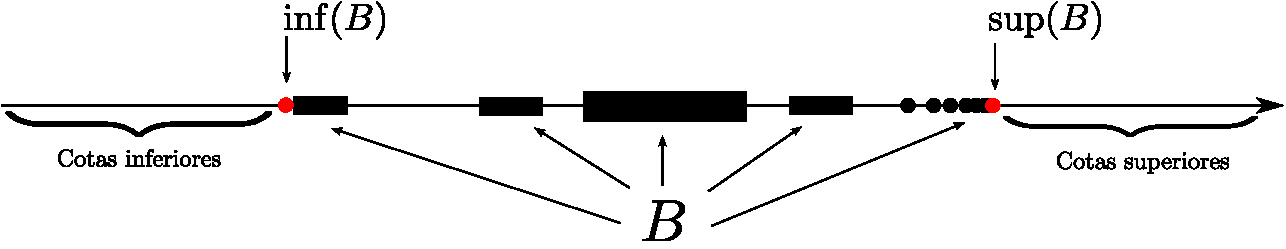
\includegraphics[width=0.98\linewidth]{Figuras/supremo-infimo}
% \caption{O supremo e o ínfimo de um conjunto $B$ limitado, representados pelo pontos indicados em vermelho. A direita indicamos os conjunto de todas as cotas superiores de $B$ e a esquerda o 
% conjunto de todas as cotas inferiores de $B$.}
% \label{fig:supremo-infimo}
% \end{figure}



% Dado um conjunto $B\subset \mathbb{R}$ defina o conjunto $-B\equiv \{-b\in\mathbb{R}: b\in B\}$.
% Então podemos verificar que se $B$ é um conjunto limitado (superiormente e inferiormente) então
% temos a seguinte igualdade 
% \[\inf(B) = - \sup(-B).\] 
% Desta forma as propriedades do ínfimo
% de conjuntos limitados podem ser obtidas por meio das propriedades do supremo e vice-versa.
% Esta equação poderia ter sido usada como definição de ínfimo. Apesar disto ter a vantagem
% de tornar a exposição mais curta, esta maneira acaba sendo pouco intuitiva para iniciantes.
% Além do mais conceitos introduzidos por negação de negação tendem a gerar bastante confusões. 

% Observamos que se levamos em conta as convenções listadas abaixo: 
% \begin{itemize}
% 	\item se $B$ não é limitado superiormente $\sup(B)=+\infty$;
% 	\item se $B$ não é limitado inferiormente $\inf(B)=-\infty$;
% 	\item $\sup \emptyset = -\infty$;
% 	\item $\inf \emptyset = +\infty$.
% \end{itemize} 
% então a igualdade $\inf(B) = - \sup(-B)$, 
% passa a ser válida para qualquer subconjunto $B\subset\mathbb{R}$.


% Por questão de conveniência relacionamos abaixo algumas propriedades do supremo e ínfimo
% que inevitavelmente serão usadas no texto. Antes, precisamos de algumas definições preliminares.
% A prova da validade das relações seguintes podem ser encontradas, por exemplo, em 
% \cite{MR0385023}. 

% \bigskip 


% Dados subconjuntos não-vazios arbitrários $A$ e $B$ contidos em $\mathbb{R}$ definimos
% \begin{itemize}
% 	\item $A+B\equiv \{ a+b\in\mathbb{R}: a\in A\ \text{e}\ b\in B\}$;
% 	\item $A\cdot C \equiv \{ a\cdot b\in\mathbb{R}: a\in A\ \text{e}\ b\in B\}$;
% 	\item $k\cdot A \equiv \{k\cdot a\in\mathbb{R}: a\in A \}$
% \end{itemize}



% \begin{teorema}\label{teo-prop-sup-inf}
% Sejam $A,B\subset \mathbb{R}$.
% \begin{enumerate}
	
% 	\item Se $A\subset B$ então $\sup(A)\leqslant \sup(B)$;
	
% 	\item Se $A\subset B$ então $\inf(B)\leqslant \inf(A)$;
	
% 	\item Se $B$ é limitado superiormente, então dado $\varepsilon>0$ existe $b\in B$ tal que 
% 	$\sup(B)<b+\varepsilon$; 
	
% 	\item Se $B$ é limitado inferiormente, então dado $\varepsilon>0$ existe $b\in B$ tal que\break
% 	$b-\varepsilon<\inf(B)$.  
	
% 	\item Se $A$ e $B$ são limitados superiormente então $\sup(A+B)=\sup(A)+\sup(B)$.
	
% 	\item Se $A$ e $B$ são limitados inferiormente então $\inf(A+B)=\inf(A)+\inf(B)$.
	
% 	\item Se $k\geqslant 0$ e $A$ limitado inferiormente então $\inf(k\cdot A)=k\inf(A)$.
	
% 	\item Se $k\geqslant 0$ e $A$ limitado superiormente então $\sup(k\cdot A)=k\sup(A)$.
	
% 	\item Se $k\leqslant 0$ e $A$ limitado superiormente então $\inf(k\cdot A)=k\sup(A)$.
	
% 	\item Se $k\leqslant 0$ e $A$ limitado inferiormente então $\sup(k\cdot A)=k\inf(A)$.
	
% 	\item Se $A,B\subset [0,+\infty)$ então $\inf(A\cdot B)= \inf(A)\cdot\inf(B)$;
	
% 	\item Se $A,B\subset [0,+\infty)$ então $\sup(A\cdot B)=\sup(A)\cdot\sup(B)$, 
% 	caso um dos conjuntos não seja limitado superiormente esta igualdade pode ser apenas  $+\infty=+\infty$.
% \end{enumerate}
% \end{teorema}

%\end{subappendices}